\documentclass[phd,tocprelim]{cornell}
%
% tocprelim option must be included to put the roman numeral pages in the
% table of contents
%
% The cornellheadings option will make headings completely consistent with
% guidelines.
%
% This sample document was originally provided by Blake Jacquot, and
% fixed up by Andrew Myers.
%
%Some possible packages to include
\usepackage{graphicx,pstricks}
\usepackage{graphics}
\usepackage{moreverb}
\usepackage{subfigure}
\usepackage{epsfig}
\usepackage{subfigure}
\usepackage{hangcaption}
\usepackage{txfonts}
\usepackage{palatino}


\usepackage{alltt}

\usepackage{algorithm}
\usepackage{multicol}
\usepackage{bbold}

\usepackage{pstricks-add}

\usepackage{algorithmic}
%\usepackage{amsmath}


%if you're having problems with overfull boxes, you may need to increase
%the tolerance to 9999
\tolerance=9999

\bibliographystyle{plain}
%\bibliographystyle{IEEEbib}

\renewcommand{\algorithmicrequire}{\textbf{Input:}}
\newtheorem{theorem}{Theorem}[section]

\newtheorem{definition}{Definition}
\newtheorem{lemma}[definition]{Lemma}
\newtheorem{corollary}[definition]{Corollary}
\newtheorem{conjecture}[definition]{Conjecture}
\newtheorem{property}[definition]{Property}

\renewcommand{\caption}[1]{\singlespacing\hangcaption{#1}\normalspacing}
\renewcommand{\topfraction}{0.85}
\renewcommand{\textfraction}{0.1}
\renewcommand{\floatpagefraction}{0.75}

\title {Community Detection in Large Networks}
\author {June Andrews}
\conferraldate {May}{2012}
\degreefield {Ph.D.}
\copyrightholder{June Andrews}
\copyrightyear{2012}

\begin{document}

\maketitle
\makecopyright


\begin{abstract}

Graphs are used to represent various large and complex networks in scientific applications.  In order to understand the structure of these graphs, it is useful to treat a set of nodes with similar characteristics as one community and analyze the community's behavior as a whole.  Finding all such communities within the graph is the object of community detection.  In our research, we compare dozens of existing community detection methods and develop a new class of algorithms for finding communities.

\end{abstract}

\begin{biosketch}
June Andrews was born in San Diego, 1985.
She attended University of California, Berkeley for her undergraduate degree in Electrical Engineering and Computer Science, with a minor in Applied Mathematics.
She is now completeing her doctoral degree in Applied Mathematics at Cornell University.
\end{biosketch}

\begin{dedication}
\begin{figure}[!h]
\centering

\includegraphics[width=3in]{Figures/windy}
\caption{\it Phil Andrews 1955 - 2011}
\end{figure}

Here's to you Da.
\end{dedication}

\begin{acknowledgements}
It goes without saying, these people have been inspiring forces of nature to work with:
\begin{itemize}
\item Len Kulbacki
\item Coach Wilson
\item James Sethian
\item Patricia Kovatch
\item John Hopcroft
\item Steve Strogatz
\item Jon Kleinberg
\end{itemize}
\end{acknowledgements}

\contentspage
\tablelistpage
\figurelistpage

\normalspacing \setcounter{page}{1} \pagenumbering{arabic}
\pagestyle{cornell} \addtolength{\parskip}{0.5\baselineskip}

\chapter{Introduction}

\section{Community Detection}

\begin{figure}[!b]
\centering
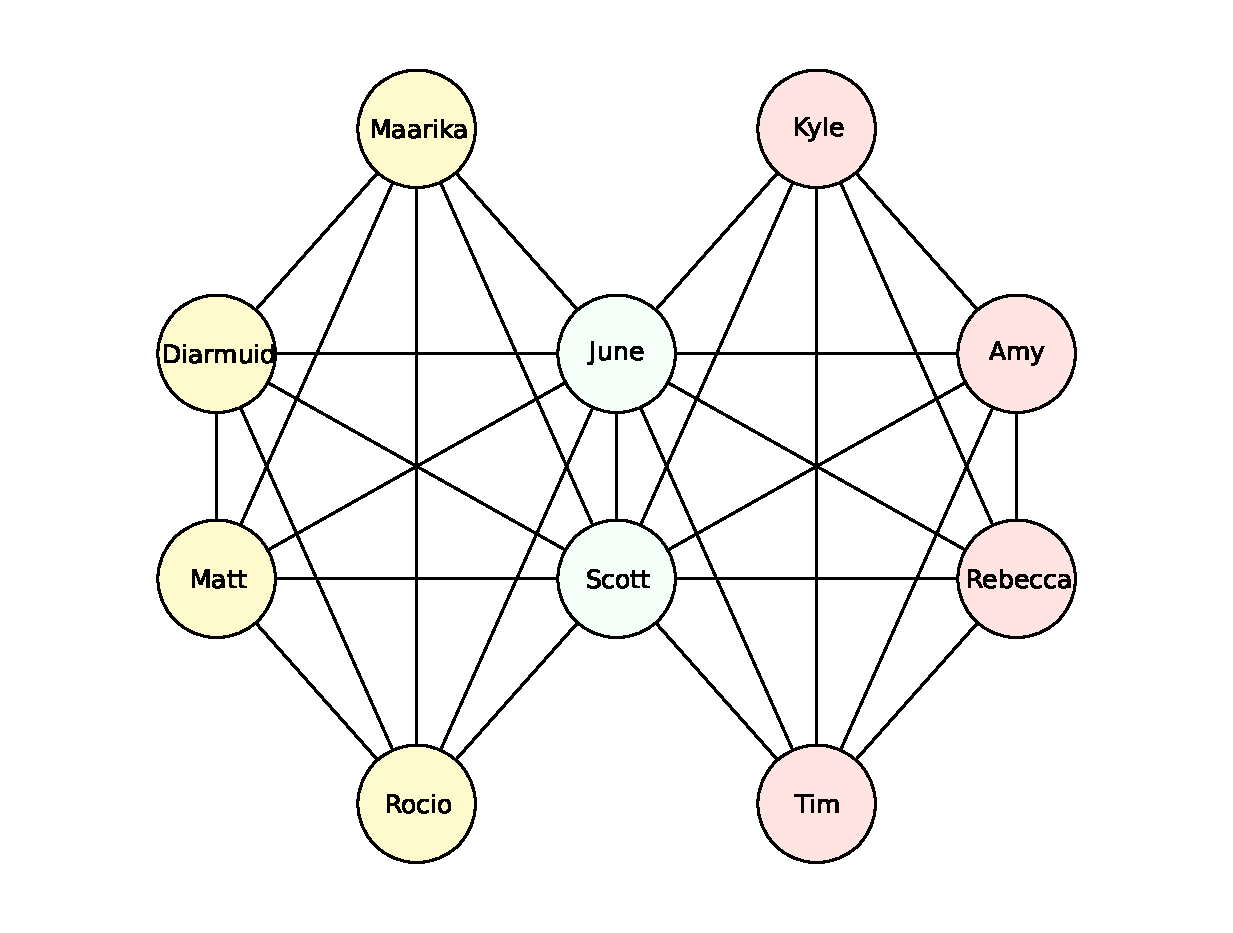
\includegraphics[width=3in]{Figures/visually_simple}
\caption{A simple graph of people and their friendships.  The graph is regular enough to reveal two communities.}
\label{fig_simple}
\end{figure}

Consider an application that studies objects and the interactions between those objects.  The application could study anything from people and their friendships, to papers and their citations; a variety of applications fall into this format.  If we let nodes represent the objects and edges represent the interactions between those objects, we can store the application's data in a graph.  While it can be possible for the application to draw conclusions by looking at every node within the graph, if the graph is large and complex, analyzing every node can be unmanageable and can produce incomprehensible results.   We simplify the graph by finding communities of nodes.  In particular, we want communities, whose members interact with each other in a particular way and interact with nonmembers of the community in a different way. If such a community is found, then two questions arise.  How are members of the community related?  How does the community interact with the rest of the graph?  Given answers to these questions, we can comprehend what is happening in the graph at a local level.  For social networks, we know that communities exist \cite{JTODO}.  Due to the large, complex nature of social networks, communities can be hard to find.  In order to find communities, we must develop the ability to see the forest through the trees.  We have to be able to extract the communities of nodes from the interactions of the graph.  This is the object of community detection.


Given a graph, there are two prominant questions community detection seeks to answer.  The first, what is a community and the second, what are the communities?  Several approaches have been developed to answer these two questions, some with a particular application as motivation.  We outline the coupling of a few sciences and one of their preferred detection methods in Table \ref{tbl_app_method}. Prior to $2002$, most development of community detection was done within the fields of the applications.  Since then, computer scientists have contributed a large volume of advances towards answering these two questions for applications in general.  The first goal of this thesis to try and tie together a portion of these advances into a cohesive understanding of community detection.  The second is to use our perspective to create fast and parallel algorithms.

\begin{table}[!h]
\centering
\begin{tabular}{l|l}
Application & Community Detection Method \\ \hline
Parallel Computation Distribution & $k-$means clustering \cite{JTODO} \\
Physics & Belief Propogation \cite{JTODO}\\
Search Queries & \cite{JTODO} \\
Sociology & \cite{JTODO} \\
Storage of Large Matrices & Spectral Analysis \cite{JTODO} \\
Taxonomy & Neighbor Joining \cite{JTODO} \\
\end{tabular}
\caption{A subset of applications and one of their preferred community detection methods.}
\label{tbl_app_method}
\end{table}


\section{Graph Partitioning Methods}

For many applications the object is to partition the graph into disjoint components.  We call each component a community.  There are an exponential number of possible partitions, but not every partition will provide useful information.  While much analysis of useful or unuseful information must be left up to the application, there are two characteristics that most applications want in communities.  The first is that nodes within a community be well connected.  The second is that the community is not well connected to the rest of the graph.  The definition of well connected is different for each community detection method.

There are two genres of finding good partitions of the graph, top down approaches that recursively cut the graph and bottom up approaches that union existing partitions.

% New section*********************************
\subsection{Top Down Approaches}
\label{sec:top_down}

Top down approaches work by recursively dividing the graph, see Algorithm \ref{alg_rec_part} for their structure.  For methods in this cateogry there are two necessary components.  The first is the ability to tell if a set of nodes $C$ is a community.  The second, if a set of nodes is not a community, then the algorithm finds a way to divide the nodes, without splitting up any communities.

\begin{algorithm}                              % enter the algorithm environment
\caption{{\sc Recursive Partitioning}}         % give the algorithm a caption
\label{alg_top_down}                                   % and a label for \ref{} commands later in the document
\begin{algorithmic}                        % enter the algorithmic environment
\REQUIRE $G=(V, E)$
\IF{ $V$ is a community}
\RETURN $V$
\ELSE
\STATE divide $V$ into $C$ and $V - C$
\RETURN $\{\mbox{\sc Recursive Partitioning}(C),\mbox{\sc Recursive Partitioning}(V-C)\}$
\ENDIF
\end{algorithmic}
\label{alg_rec_part}
\end{algorithm}

% new section**************
\subsubsection{Conductance}

Conductance is a measure of a cut within the graph developed by JTODO \cite{JTODO}.  For a given cut, if conductance is low, then there are relatively few edges crossing the cut.  Inutitively, this implies that the cut does not divide a community.  If further divisions do not improve conductance, then we have found a community.

\begin{equation}
\mbox{\sc Conductance}(C) = \frac{\sum\limits_{u \in C, v \notin C} w(u,v)}{\sum\limits_{u \in C, v \notin C} w(u,v)  + \sum\limits_{u,v \in C} w(u, v)}
\end{equation}

While this algorithm is not in heavy use, conductance is used as a measure of whether or not other algorithms that cut the graph have split a community.

% new section**************
\subsubsection{Betweenness and Centrality Measures}

Betweenness and centrality measures were first presented by Givan and Newman \cite{girvan}.  The intuition is, if an edge lies between two communities, then several shortest paths between nodes of the two communities will traverse the edge.  We remove these edges to divide the network into components.  When there are no preferential edges for shortest paths within a component, there are no more edges between communities, and the component is a community.

% new section**************
\subsection{Bottom Up Approaches}
\label{sec:bottom_up}

Bottom up approaches work by unioning together subsets of nodes until the subset is a community.  See Algorithm \ref{alg_rec_union} for their structure.  For algorithms in this category there are two components.  The first is the determination of which subsets to union.  The second is the determination of when a set of nodes is a community.  To accomplish these, most bottom up approaches use a metric over the set of subsets.  If no two subsets can be unioned to increase the metric then, every subset is a community.

\begin{algorithm}                              % enter the algorithm environment
\caption{{\sc Recursive Unioning}}         % give the algorithm a caption
\label{alg_bottom_up}                                   % and a label for \ref{} commands later in the document
\begin{algorithmic}                        % enter the algorithmic environment
\REQUIRE $S = \{C_1, C_2, \dots \}$
\IF{There exists $C_i$ and $C_j$, such that $C_i \cup C_j$ is a community}
\RETURN {\sc Recursive Unioning}$(\{S - C_i - C_j\} \cup \{C_i \cup C_j\})$
\ELSE
\RETURN $S$
\ENDIF
\end{algorithmic}
\label{alg_rec_union}
\end{algorithm}

% new section**************
\subsubsection{Modularity}

The overwhelmingly popular metric in this category is modularity.  Modularity was first presented by Newman \cite{newman}.  The metric measures the distance between a provided set of communities and a randomly generated set of communities.  Maximizing modularity finds the least random set of communities.

Fast algorithms have been developed for maximizing modularity.  In this paper we use the Louvain Algorithm developed by Blondel et. al\cite{blondel}.  The same fast algorithm can be used for the similar metric, modularity ratio \cite{JTODO}.

% new section**************
\section{Overlapping Community Detection}

We call two communities overlapping, if there exists a node that is a member of both communities.  In practice, these communities are common.  For example, think of the community of your colleagues and the community of your family. You are a member of both communities, and while they are different communities, they are overlapping.  In fact, for most social networks, we expect there to be many overlapping communities.


% new section**************
\subsection{Alpha Beta Clustering}

In previous sections, communities were the partitions of a graph.  Each node was placed in exactly one community.  So if it was optimal to place node, $n$, in community $C_1$, then node $n$ would not be placed in community $C_2$.  Alpha beta clustering makes a change to this step.  If adding node $n$ to community $C_2$ has a high value, alpha beta clustering adds node $n$ to community $C_2$, as well as $C_1$.  This simple change dramatically restructures community detection.  The new structure is a two part process:
\begin{enumerate}
\item Create a definition of a community that does not depend on other communities in the graph.
\item Find each community seperately.
\end{enumerate}

We now present Mishra's et al \cite{mishra} approach following these guidelines.  Let us say the strength of a connection between a node and a community is the number of edges the node has to members of the community, denoted as $|E(n, C)|$.  See Table \ref{table_variables} for a list of all notation. Mishra et al \cite{mishra} use this notion of strength to define a community satisfying the first guideline.  In particular, no node outside of the community is more strongly connect to the community than any of the nodes inside the community.  Here is the formal definition of an $(\alpha, \beta)$ community.
\begin{definition}[$(\alpha, \beta) - $ Community]
For community $C$, let:
\begin{eqnarray*}
\alpha(C) &=& \min\limits_{n \in C} |E(n, C)|\\
\beta(C) &=& \max\limits_{n \notin C} |E(n, C)|
\end{eqnarray*}
If $\alpha(C) > \beta(C)$, then $C$ is an $(\alpha, \beta)$ community.
\end{definition}

Given this definition, Mishra et al\cite{mishra} are able to find communities quickly and in parallel.  In our development of a parallel algorithm we use the same guidelines.

\section {More Approaches}

So far, we have introduced the community detection methods that have provided inspirations for this thesis.  There are countless more methods.  We briefly outline the most prominent of those methods.

\begin{itemize}
\item Kernighan-Lin Algorithm
\item $k$-Clique Percolation
\item Belief Propogation
\item Heirarchy methods
\item Principle Component Analysis
\end{itemize}


\section {Desired Improvements}

In the field of community detection both algorithms and data sets are increasing in complexity.  Hence, a useful theoretical result is the ability to compare and understand complex algorithms.  Additionally, a useful experimental result is the ability to compute overlapping communities in parallel on large networks.

We deliver on the these results:
\begin{itemize}
\item A framework for comparing existing community detection methods.
\item A community definition encouraging overlapping communities.
\item A parallel algorithm with near perfect scalability to analyze large networks.
\end{itemize}


\section{Notation}

We use the same notation throughout the thesis. A brief description of variables is listed in Table \ref{table_variables}. 

The assumptions we make are:
\begin{itemize}
\item {\it Self-Loops.}  We presume there are no self loops in the networks.  As a node will always be in the same community as itself, self-loops provide redundant information.  Accordingly, $w(u, u) = 0$, for all $u \in V$.  We note that this assumption is not held in some of the literature we reference.
\item {\it Edges} We presume that all edges exist and are weighted between $0$ and $1$.  The edge weight function is $w : VxV \rightarrow \mathbb{R}_{[0, 1]}$  Unweighted graphs can easily be adapted into this notation.
\end{itemize}

We also introduce internal and external edges.
\begin{definition}[Internal Edges]
Internal edges are edges between members of the same community $C$.
\end{definition}
\begin{definition}[External Edges]
External edges are edges between a member of community $C$ and a nonmember of $C$.
\end{definition}

\begin{table}
\caption{Notation}
\begin{center}
\begin{tabular}{|c|c|c|} \hline
Variable Name & Description & Constraints \\ \hline
$V$ & Set of all nodes within the network & $\{u | u \in \mbox{ the network }\}$\\ \hline
$u$ and $v$ & Nodes & $u, v \in V$ \\ \hline
$w(u,v)$ & Edge Weight Function &  $w:VxV \rightarrow \mathbb{R} _{[0, 1]}$ \\ \hline
$G$ & Network or Graph & $G(V,E)$ \\ \hline
$C$ & Community & $C \subset V$ \\ \hline
$k$ & Fraction of nodes within $C$ & $k = \frac{|C|}{|V|}$ \\ \hline
$|C|$ & Size of $C$ & $|C| = k|V |$ \\ \hline
$S$ & Set of Communities & $S = \{C_1,C_2,\dots,C_n\}$\\ \hline
\end{tabular}
\end{center}
\label{table_variables}
\end{table}

\begin{table}
\caption{Introduced Functions}
\begin{center}
\begin{tabular}{|c|c|} \hline
Function & Description \\ \hline
$I(C)$ & Internal Density of a single Community, $C$, Definition \ref{def_int_density} \\ \hline
$E(C)$ & External Density of a single Community, $C$, Definition  \ref{def_ext_density} \\ \hline
$I(S)$ & Internal Density of a set of Communities, $S$, Definition \ref{def_int_set} \\ \hline
$E(S)$ & External Density of a set of Communities, $S$, Definition \ref{def_ext_set} \\ \hline
{\sc Conciseness}$(S)$ & Conciseness of a set of Communities, $S$, Definition \ref{def_conciseness} \\ \hline
\end{tabular}
\end{center}
\label{table_new_functions}
\end{table}





% New Chapter
\chapter{A Framework for the Comparing Metric Based Detection Methods}

There are a variety of community detection metrics and they are difficult to compare.  To date only experimental methods have been available to analyze them.  Lancichinetti and Fortunato \cite{lanc:2009} found [algorithms that optimize metrics] work better on certain networks.  Leskovec et. al \cite{leskovec} found as community size increases, the communities that optimize certain metrics diverge from our understanding of a strong community.  The pattern for comparing metrics is to begin with a set of metrics, a set of algorithms to optimize each metric, and a network.  Communities found by the algorithms are then compared via their characteristics.  Characteristics include: diameter, average path length, degree distribution, size, internal density, etc.

Our approach is the reverse of previous comparisons.  We begin with considering the characteristics of a community.  The possible values of these characteristics create a multidimensional space.  Metrics collapse this multidimensional space onto the real numbers.  We can then categorize the multidimensional space according to how the metric evaluates communities with certain characteristic values.  In this sense we can get a theoretical understanding of metrics.  We follow through with experiments on four networks to confirm our findings.


% New Section*****************
\section{Previous Comparisons}







Communities are defined by two characteristics, members of the community interact with each other in a particular way and interact with nonmembers of the community in a different way.  Generally, a community is accepted as a set of nodes that interact frequently with each other and interact infrequently with nonmembers of the community.  The first characteristic corresponds to a high internal density, see Definition \ref{def:int_density_single}.  The second corresponds to a low external density, see Definition \ref{def:ext_density_single}.  Detection methods vary in their formulation of density and their prioritization of finding communities with higher internal density verse lower external density.

All known comparisons have been experimental.  The experiments are run by first selecting a set of networks.  Then, each detection method finds the communities within each network.  Finally, using a set of metrics the communities found by each method are compared.  Lancichinetti and Fortunato \cite{lanc:2009} compared three popular partition algorithms with generated graphs and used normalized mutual information as the comparison metric.  Their results conclude that partition algorithms are fast and work well for non-overlapping communities.  Leskovec et. al \cite{leskovec} conducted a broader study.  They used eight classes of algorithms over $40$ networks and compared the results with a series of metrics covered in this chapter.


% New Section******************************
\section{Community Characteristics}

Each characteristic of a community is a dimension in the multidimensional space that a metric compresses.  Here is a sampling of the more common characteristics of a community.
\begin{itemize}
\item {\sc Internal Density} is density of edges within the community.
\item {\sc External Density} is the density of edges leaving the community.
\item {\sc Size} is the number of nodes within the community.
\item {\sc Diameter} is the longest, shortest path between any two members of the community.
\item {\sc Average Shortest Path} is the average shortest path between any two members of the community.
\item {\sc Out Degree Fraction} is the fraction of a node's edges leaving the community.
\item {\sc Degree Distribution} is the distribution of the degrees of nodes within the community.
\end{itemize}
There are many more specific characteristics, but we find that a community can be well described by the above list.  The listed characteristics are not independent.  A high internal density indicates a small diameter and short average path length.  A low external density limits the out degree fraction.  In fact, the value of most characteristics can be bounded by internal and external density values.  The size of a community can not be.  Hence, the characteristics of internal density, external density, and community size capture a large amount of information about a community's set of characteristics.  We will use this to our advantage and simplify our analysis by only using these three characteristics: internal density, external density, and size.


% New Section*******************************
\section{Individual Community Based Metrics}

Here, we explore metrics that evaluate the strength of a single community.  There are three uses of such metrics.  The first is for use in a Top Down (Section \ref{sec:top_down}) or Bottom Up style (Section \ref{sec:bottom_up}) style algorithm to find a partitioning of the network.  The second is to find a single community within the network.  The third is to compare communities found by complex detection techniques.  The later use is more common for these metrics, of which conductance is the most popular \cite{JTODO}.


% New subsection********************************
\subsection{Internal and External Density}

The most distinct community is a clique, disconnected from the rest of the graph.  The internal density is maximized and the external density is minimized.  Formal definitions follow.

\begin{definition}[Internal Density]
\label{def:int_density_single}
Internal density is the total weight of edges that exist between members of the community, {\it internal edges}, compared to the total possible weight that could exist within the community.  Hence, $I(C) : C \rightarrow \mathbb{R}_{[0, 1]}$, where
\begin{equation}
 I(C) =\frac{\sum_{u \in C} \sum_{v \in C} w(u,v)}{|C|(|C| - 1)} .
\end{equation}
\label{def_int_density}
\end{definition}

For a community $C$ that has no edges between its members, the {\it internal density} will be minimized with, $I(C) = 0$.  For a community $C$ that is a clique, {\it internal density} will be maximized with $I(C) = 1$.  The closer a community, $C$ is to an {\it internal density} value of $1$, the close it is to being a clique.  

\begin{definition}[External Density]
\label{def:ext_density_single}
External density is the total weight of edges that exist between a member of the community and a nonmember of the community, {\it external edges}, compared to the total possible edge weight that could exist leaving the community:
\begin{equation}
 E(C) = \frac{\sum_{u \in C} \sum_{v \notin C} w(u,v)}{|C|(|V| - |C|)}.
\end{equation}
\label{def_ext_density}
\end{definition}

For a community $C$ that has all possible {\it external edges}, external density will be maximized at $E(C)=1$.  For a community $C$, disconnected from the rest of the graph, external density will be minimized at $E(C) = 0$.

There are other representations of $I(C)$ and $E(C)$ that vary how the $|C|$ and $|V|$ terms are used.  The analysis and conclusions that follow are not sensitive to such variations.

With our parameterization, all communities can be mapped to a point $(I(C), E(C))$ in the square $\mathbb{R}_{[0, 1]} x \mathbb{R}_{[0, 1]}$.   Communities with certain values do not correspond to our understanding of a strong community.  Such values are $\left(0, \frac{1}{2}\right)$, $\left(\frac{1}{2}, 1\right)$, etc.  However, a community mapped to $\left(\frac{1}{2}, 0\right)$ corresponds to a strong community.  We define the strongest possible community to be ideal.
\begin{definition}[Ideal Single Community]
A community, $C$, is ideal if it is an isolated clique, specifically has the following properties:
\begin{eqnarray*}
I(C) &=& 1\\
E(C) &=& 0.
\end{eqnarray*}
\end{definition}


% New subsection********************
\subsection{Study of Relevant Metrics}

Given that we can map a community, $C$, to the point $(I(C), E(C))$, we now analyze how different metric based detection methods operate in the $I,E$ plane.  We cover six metrics that evaluate a single community.  We use one approximation to simplify the equations, $|C| \approx |C| - 1$.  This approximation has a larger impact on smaller communities, but most communities of interest are large enough to allow the approximation.  Additionally, we introduce variable, $k$, representing the portion of the nodes within community, $C$, such that $|C| = k |V|$
\begin{itemize}
\item {\sc Conductance} is the probability that a step in a random walk will leave the community \cite{JTODO}.
\begin{equation}
\mbox{\sc Conductance}(C) = \frac{(1 - k)E(C)}{kI(C) + (1 - k)E(C)}
\end{equation}
\item {\sc Cut Ratio} is the fraction of existing to possible edges leaving the community \cite{JTODO}.
\begin{equation}
\mbox{\sc Cut Ratio} = E(C)
\end{equation}
\item {\sc Edges Cut} is the number of edges connecting the community to the rest of the graph \cite{JTODO}.\begin{equation}
\mbox{\sc Edges Cut} = k (1-k) |V|^2 E(C)
\end{equation}
\item {\sc Expansion} the average number of edges leaving the community per node \cite{JTODO}.
\begin{equation}
\mbox{\sc Expansion} = (1 - k)|V |E(C)
\end{equation}
\item {\sc Internal Density} as a metric, previously existed before our definition of $I(C)$, \cite{JTODO}.  However, we stick to our definition of $I(C)$ for intutive reasoning and note in previous work internal density represents the mirror image of our definition.
\begin{equation}
\mbox{\sc Internal Density} = 1 - I(C)
\end{equation}
\item {\sc Volume} is the total degree of nodes within the community \cite{JTODO}.
\begin{equation}
\mbox{\sc Volume} = |C|^2 I(C) + k(1-k)|V|^2E(C)
\end{equation}
\end{itemize}
 With this parameterization of the metrics, we can already draw some conclusions.  All metrics, besides {\sc Volume} and {\sc Conductance} are a function of either $I(C)$ or $E(C)$, but not both.  A metric that considers only $I(C)$ will be optimized by any clique.  Which is a very restrictive definition of a community and finding all communities in the graph under such a definition is equivalent to finding all the cliques in a graph, a NP-hard problem.  A metric that considers only $E(C)$ will be optimized by any disconnected component of the graph, including a community that includes the entire graph.  While it is possible to find all disconnected components in linear time, it also provides no information about most datasets.

For the metrics that can be parameterized in terms of $I(C)$ and $E(C)$, we can use level sets.  Level sets are a way to visually categorize a space.  Let us pick the metric conductance.  An optimal value of conductance is $0$.  We can find all points of $(I(C), E(C))$ (without knowing $C$) that evaluate to {\sc Conductance}$(C) = 0$.  These points form a line in the $(I, E)$ space.  Now, we find all the points of $(I(C), E(C))$ that have a conductance value of {\sc Conductance}$(C) = \delta$.  These points will also form a line in the $(I, E)$ space.  Because of the continuity of conductance, any community, $C$, that evaluates to an $(I, E)$ point that lies between these two lines must have a conductance value of {\sc Conductance}$(C) \in (0, \delta)$.  In this way we can visually categorize the space.

\begin{figure}
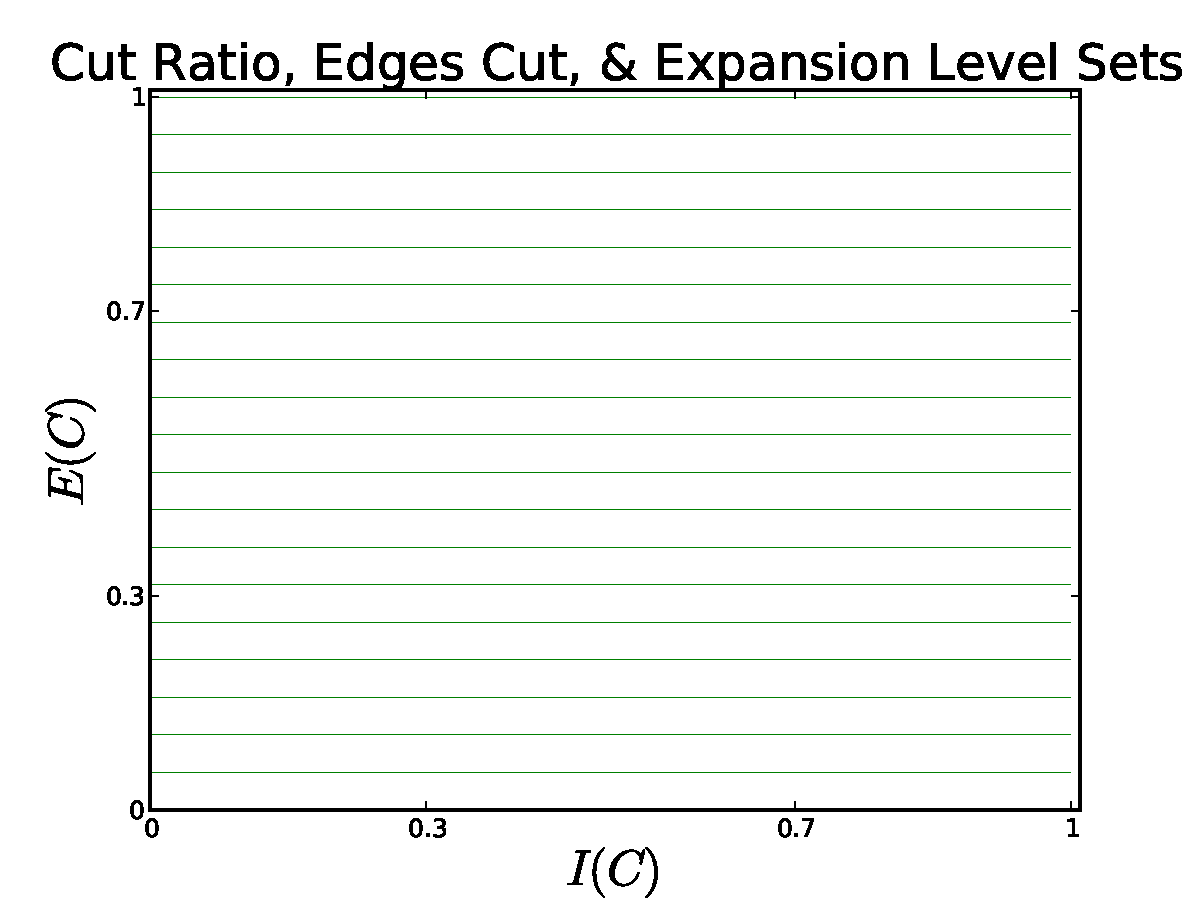
\includegraphics[width=3in]{Figures/e_based_ls}
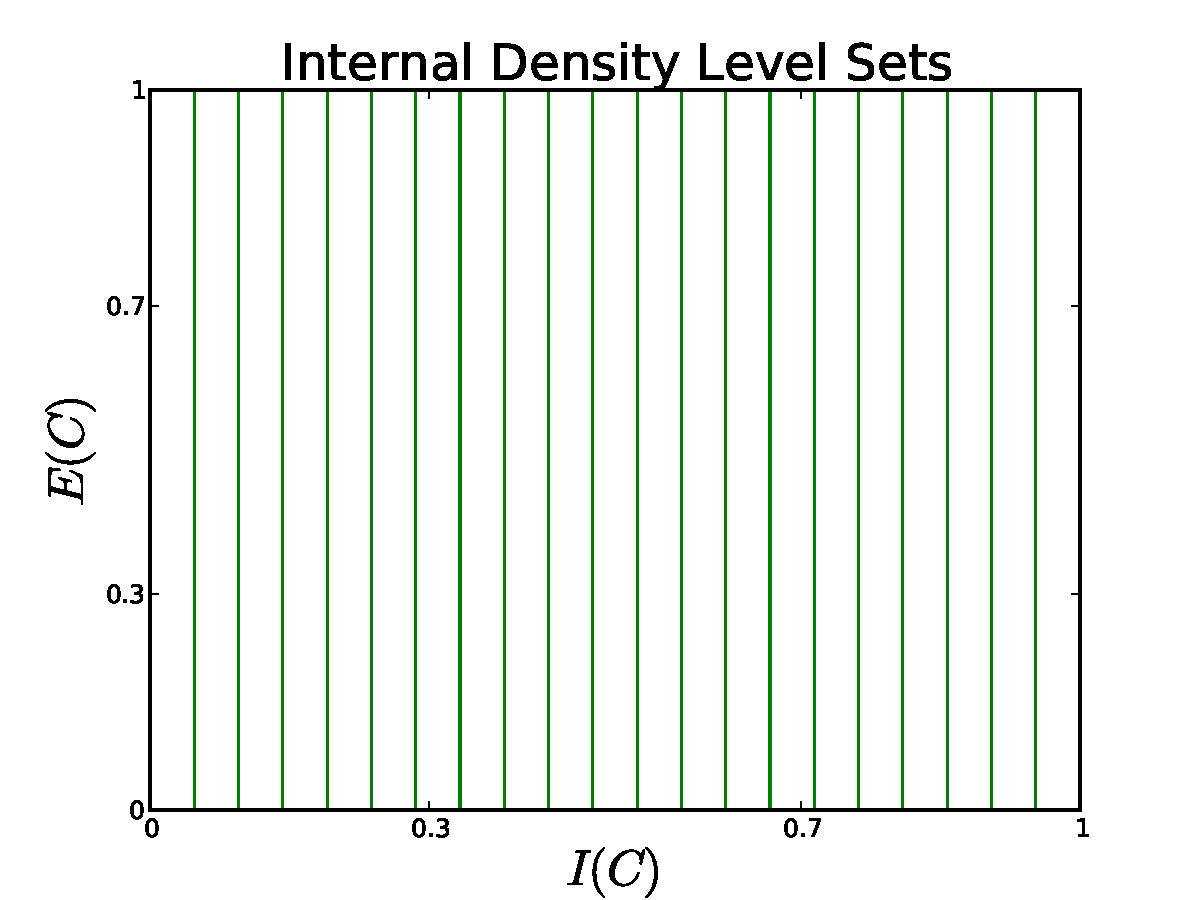
\includegraphics[width=3in]{Figures/prev_int_ls}
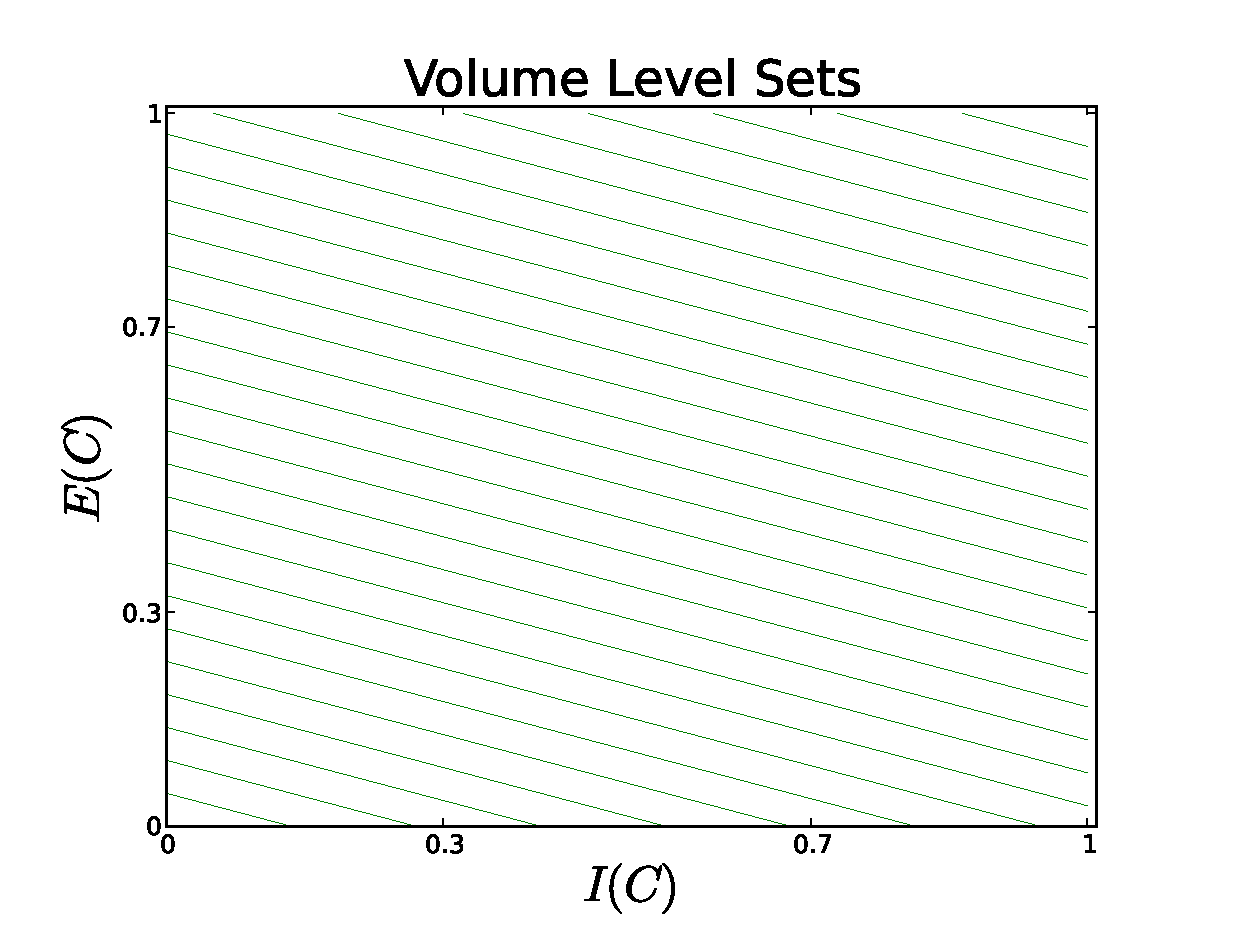
\includegraphics[width=3in]{Figures/volume_ls}
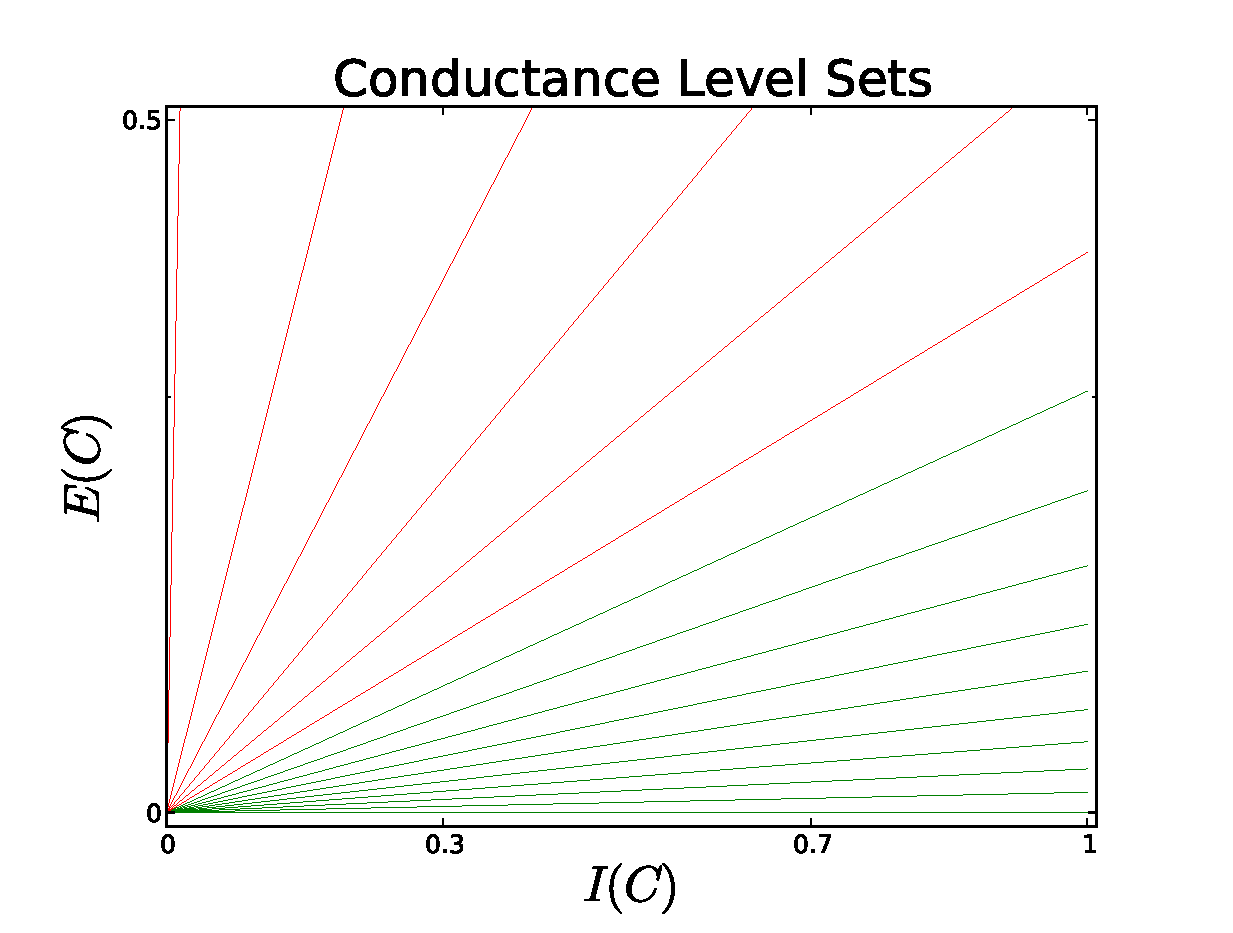
\includegraphics[width=3in]{Figures/cond_ls}
\caption{Level Sets in the $(I, E)$ plane for different metrics of a single community.  There are four ways the $(I, E)$ space is categorized.}
\label{fig_single_ls}
\end{figure}


 In level set figures, any two points in the $I,E$ plane connected by a curve have the same metric value. In our Greedy Algorithm \ref{alg_greedy_single}, if the algorithm can add a node to the community that crosses a level set to a higher metric valuation, the algorithm will add that node.  Visually, the more level sets crossed by a change to the community, corresponds to a higher change in the metric.  Traditionally, level sets are used in this manner to show gradient descent to find a local minimum.  The optimum that a gradient descent will find, can be found by traveling perpendicular to the level sets.  While we find in practice this is a good analogy to understand the behavior of optimizing these metrics,  we can not complete the analogy as the metrics are discrete.

While it is possible to draw conclusions now from the level sets, we proceed with finding communities based on these metrics.  In doing so, we confirm and expand experimental results.


\begin{table}[!h]
\centering
\begin{tabular}{|c | c  c  |}
 \hline Metric & Optimal $C$ & $(I(C), E(C))$ \\ \hline
{\sc Conductance} & $G$& $(x, 0)$\\ \hline
{\sc Cut Ratio}  & $G$ & $(x, 0)$\\ \hline
{\sc Edges Cut}  & $G$& $(x, 0)$ \\ \hline
{\sc Expansion}  & $G$&$(x, 0)$ \\ \hline
{\sc Internal Density}  & any clique & $(1, x)$ \\ \hline
{\sc Volume}  & $G$& $(x, 0)$ \\ \hline
\end{tabular}
\caption{Communities that optimize each metric.  A value of $x$, indicates that the optimization is independent of that value. }
\label{tbl_single_optimal_communities}
\end{table}


% subsubsection*************************************
\subsubsection{Greedy Algorithm}

The Greedy Single Community Metric Optimization Algorithm \ref{alg_greedy_single} takes as input a community and a metric.  The algorithm then expands the community, one node at a time, until the metric can not be improved.  The resultant community is a local optimum of the metric.

\begin{algorithm}                              % enter the algorithm environment
\caption{{\sc Greedy Single Community Metric Optimization}}         % give the algorithm a caption
\label{alg_greedy_single}                                   % and a label for \ref{} commands later in the document
\begin{algorithmic}                        % enter the algorithmic environment
\REQUIRE $C$, $G=(V, E)$, and {\sc Metric}
\STATE $inc = 1$
\WHILE{$inc \geq 0$ and $C \neq V$}
\STATE Let $u \in V$ maximize {\sc Metric}$(C \cup u)$.
\STATE $inc \leftarrow$ {\sc Metric}$(C \cup u) - $ {\sc Metric}$(C)$
\STATE $C \leftarrow C \cup u$
\ENDWHILE
\RETURN $C$
\end{algorithmic}
\end{algorithm}

Some metrics require minimization rather than maximization, this algorithm can be adapted accordingly.
In the following sections, we use the algorithm by starting with a metric and a subset of two connected nodes.  The algorithm produces a series of nested communities, each with an increasing metric score.  For each nestled community, we compute their $(I(C), E(C))$.  This gives us a path through the $(I, E)$ plane.  We can use level sets to explain the pattern of node selection that increases the metric.


% subsubsection*************************************
\subsubsection{Expansion, Edges Cut, and Cut Ratio}

We now consider metrics that are functions of $E(C)$ and not of $I(C)$: {\sc Expansion}, {\sc Edges Cut}, and {\sc Cut Ratio}.  To understand these metrics we plot how they categorize the $(I, E)$ plane with level sets and how iterations of the greedy algorithm choose communities in the $(I, E)$ plane.

For these three metrics, their definitions vary, but their level sets are identical, as shown in Figure \ref{fig_single_ls}.   The level set of $E(C) = 0$ corresponds to the metric's optimal set of communities.  These communities that are disconnected from the rest of the graph, and can have an arbitrary internal density.  These metrics favor decreases in external density over increases in internal density.  In fact, for a community at any position in the $(I, E)$ plane, the node that decreases external density the most will be choosen by the greedy algorithm, rather than a node that improves internal density.  The effect of which is visible in the greedy algorithm's path through the $(I, E)$ plane.

\begin{figure}[!h]
\centering
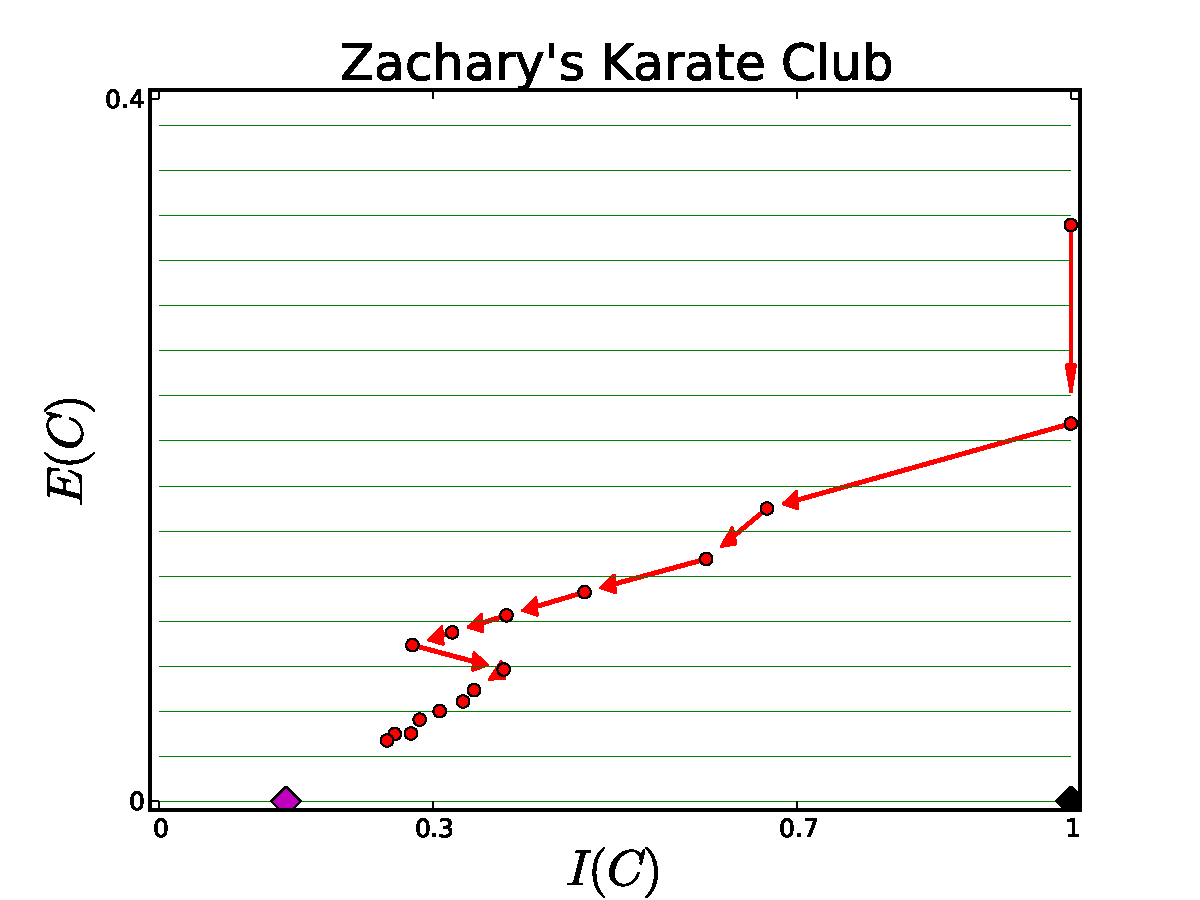
\includegraphics[width=2.8in]{Figures/cee_karate}
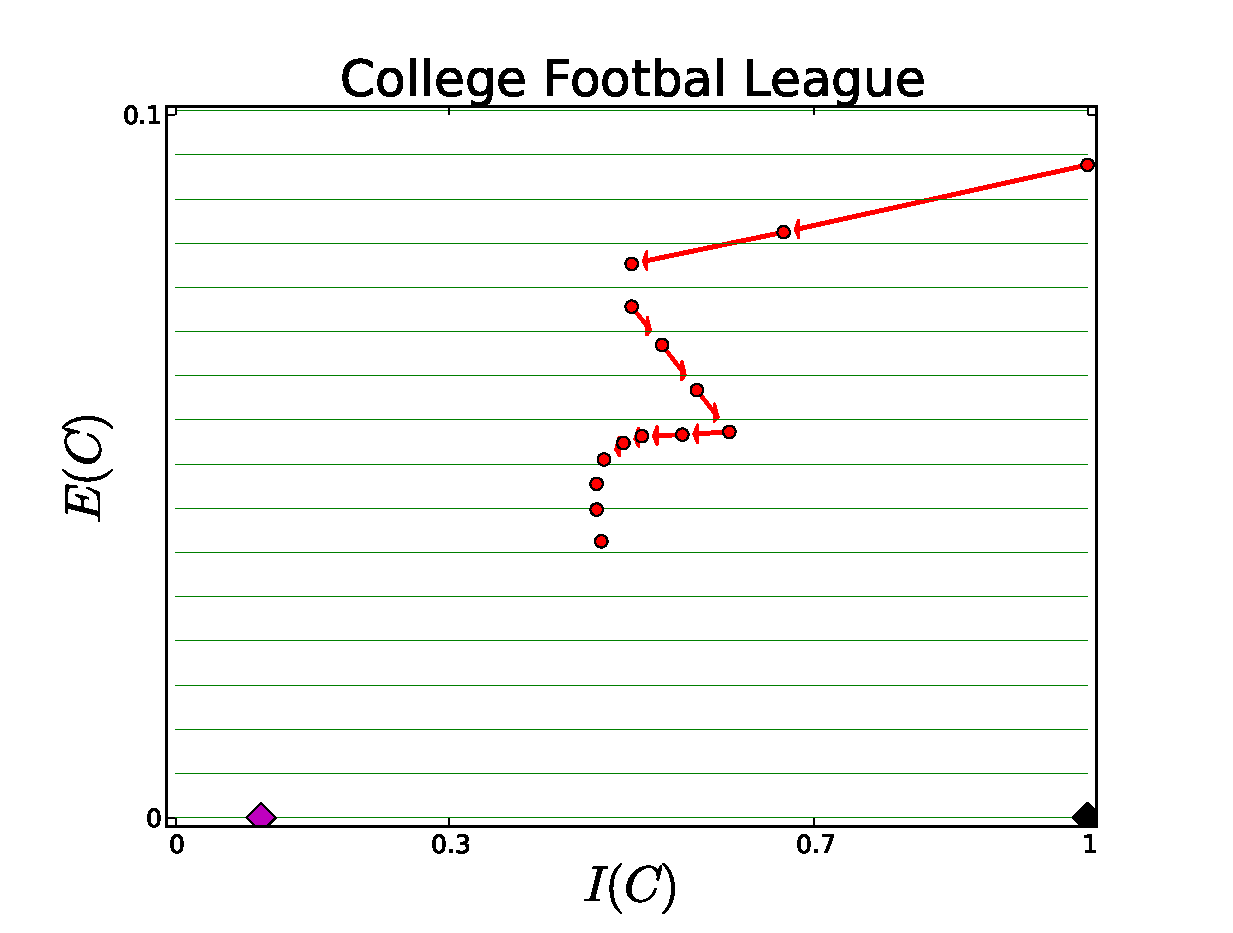
\includegraphics[width=2.8in]{Figures/cee_cfl}
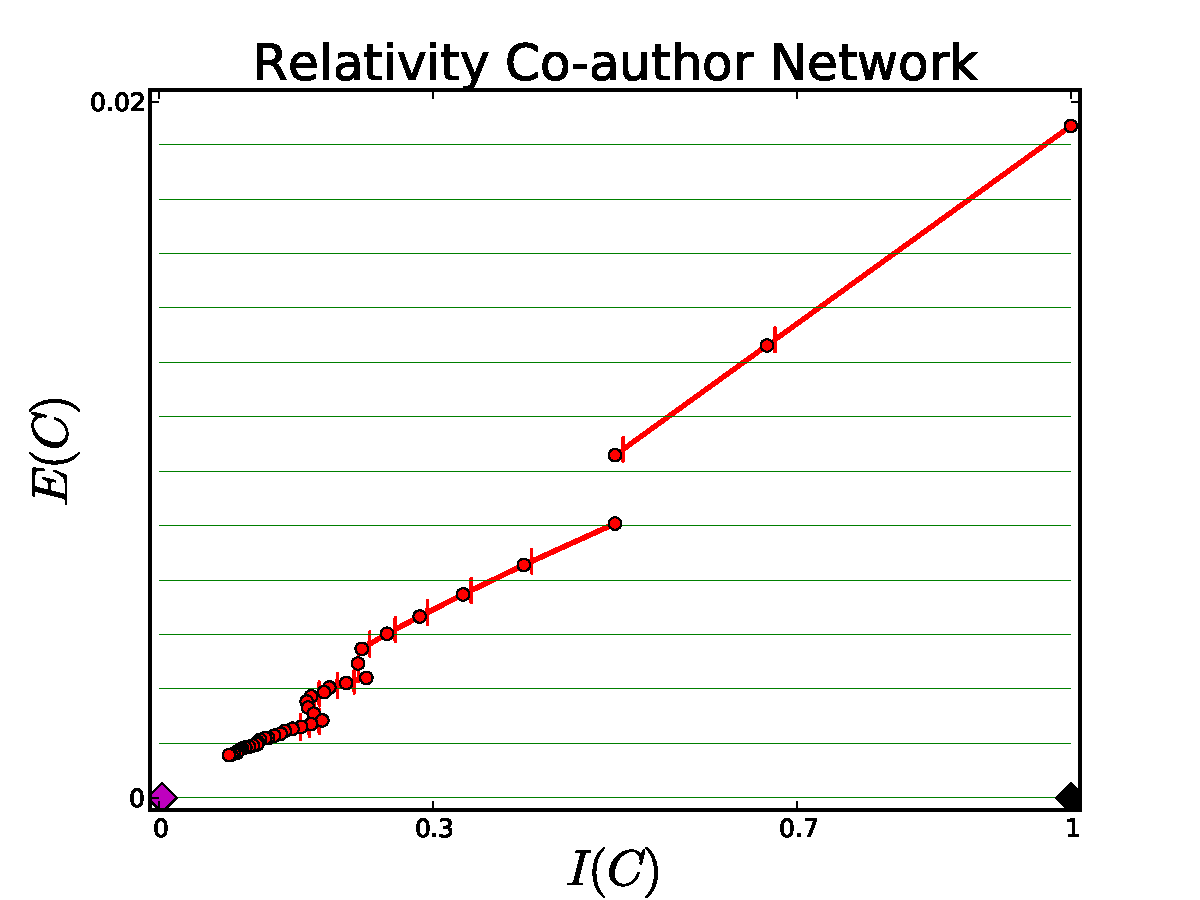
\includegraphics[width=2.8in]{Figures/cee_relativity}
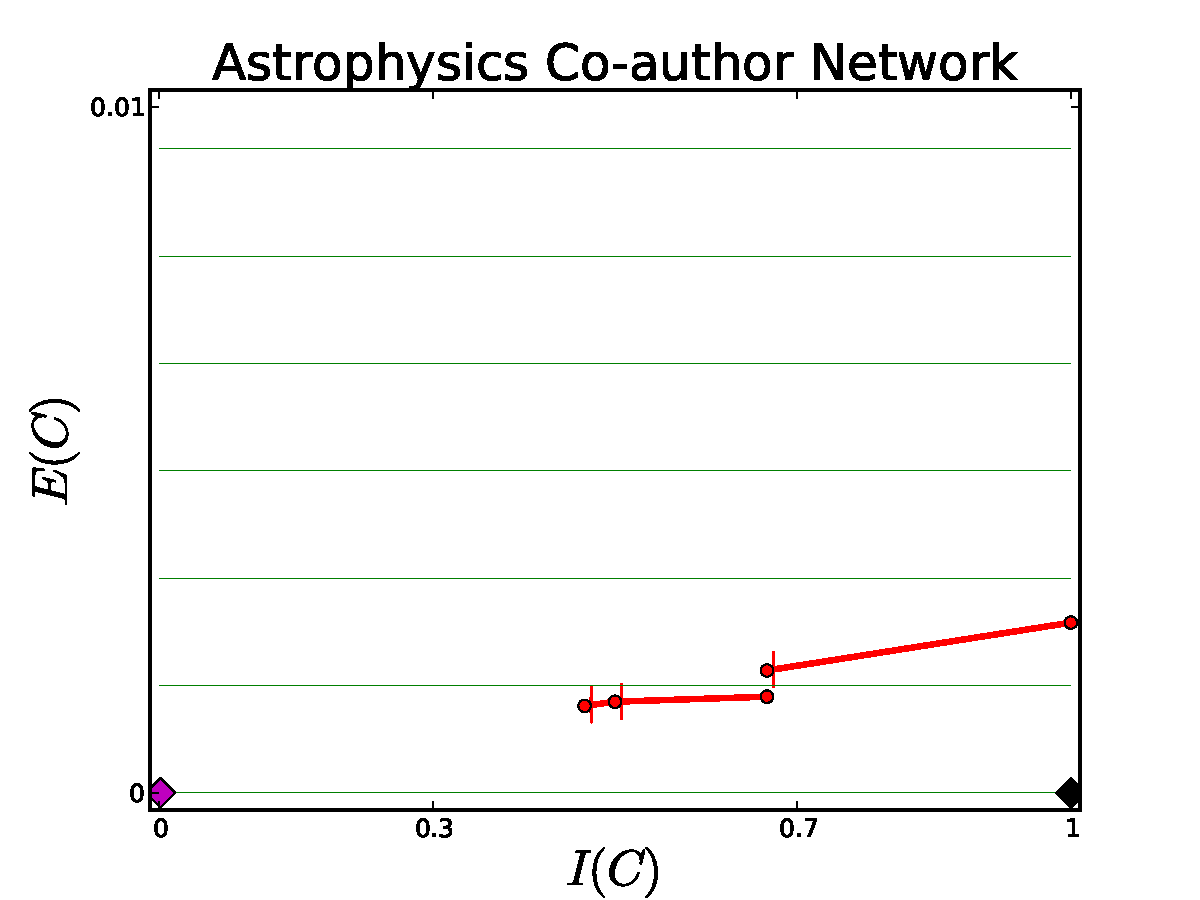
\includegraphics[width=2.8in]{Figures/cee_astro}
\caption{External Density based metrics({\sc Cut Ratio}, {\sc Edges Cut}, and {\sc Expansion}) optimized in different networks.  The lower left diamond is the $(I(C), E(C))$ point corresponding to a community of the entire graph.  The lower right diamond is the $(I(C), E(C))$ point corresponding to an ideal community.  The path corresponds to the intermediatory $(I, E)$ values of adding nodes that optimize the metrics using Greedy Algorithm \ref{alg_greedy_single}}
\label{fig_real_e_based}
\end{figure}

Because all of these metrics only respond to changes in external density, the order of nodes the greedy algorithm adds to the community does not vary between the three metrics.  The difference between the three metrics is when they terminate.  Termination in this case is determined by the size of the community, $k = \frac{|C|}{|V|}$.  Cut ratio is unresponsive to changes in the size of the community, while expansion linearly discounts against larger communities.  Edges cut heavily favors very large or very small communities.  See {\it Fig. \ref{fig_k_e_based}}.  

\begin{figure}[!h]
\centering
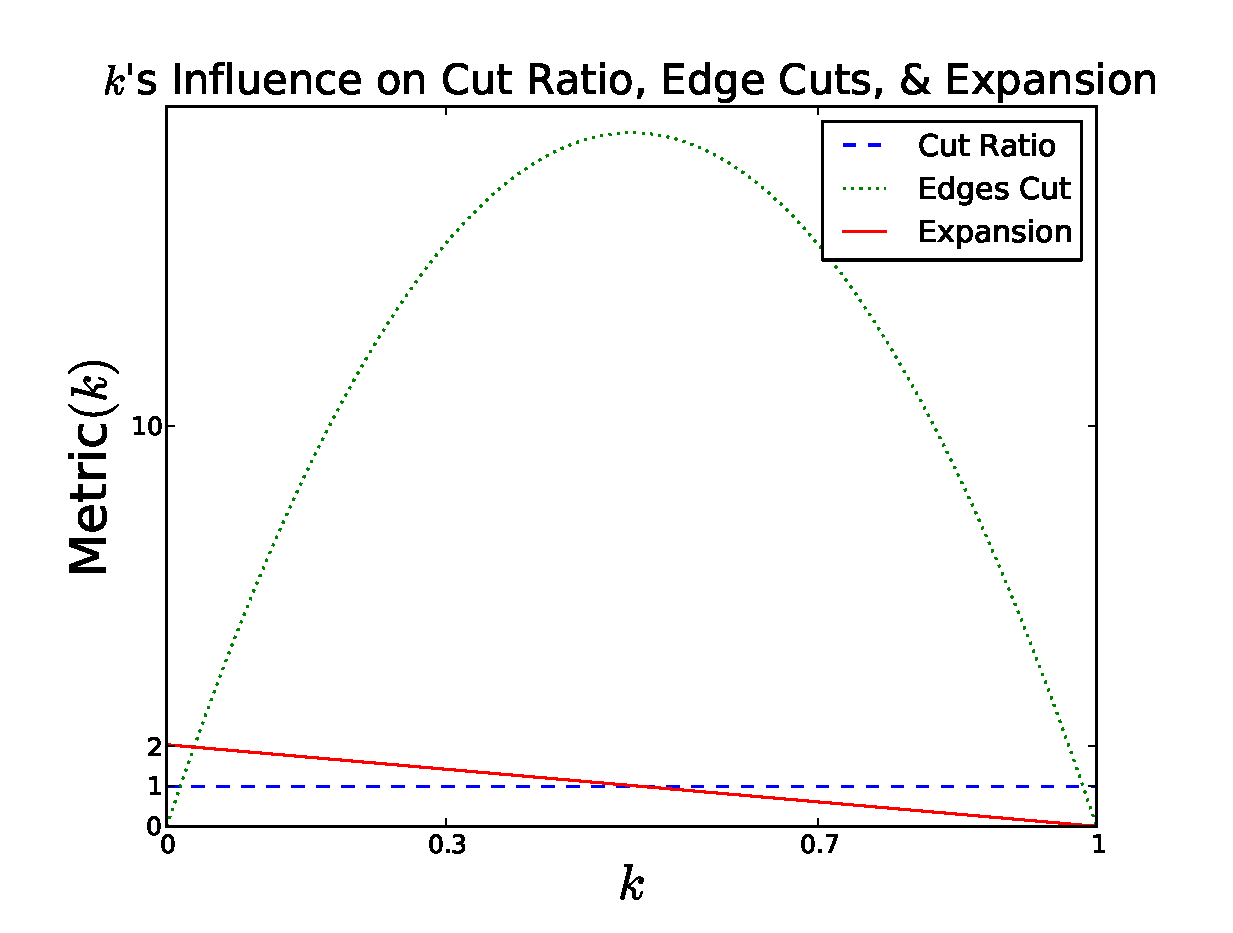
\includegraphics[width=4in]{Figures/k_influence_e_based}
\caption{Influence of size of community on the values of external density based metrics.}
\label{fig_k_e_based}
\end{figure}




% subsubsection*************************************
\subsubsection{Internal Density as Previously Defined}

Internal density is a function of internal density and is unresponsive to changes in the the external density.  Hence, only cliques and subsets of cliques optimize internal density. We do not include indepth analysis, but rather a summary.  The level sets of internal density are vertical lines in the $I,E$ plane, as seen in Figure \ref{fig_single_ls}.  The greedy algorithm augments our input of two connected nodes to the largest clique it can find(if forced to), as two connected nodes are already a clique.


% subsubsection*************************************
\subsubsection{Volume}


A metric that takes both internal and external density into account is volume.  The next conclusion is not apparent just from the equation parameterized in terms of internal and external density.  However, observing the level sets of volume reveal that the optimal community is at $(I, E) = (0, 0)$ and volume as a metric is optimal for communities with low external density and low internal density.  Apart from communities of unconnected nodes, volume can best be optimized by a community encompassing the entire graph.  Volume contradicts our intuition that communities should have good internal connectivity.

\begin{figure}[!tb]
\centering
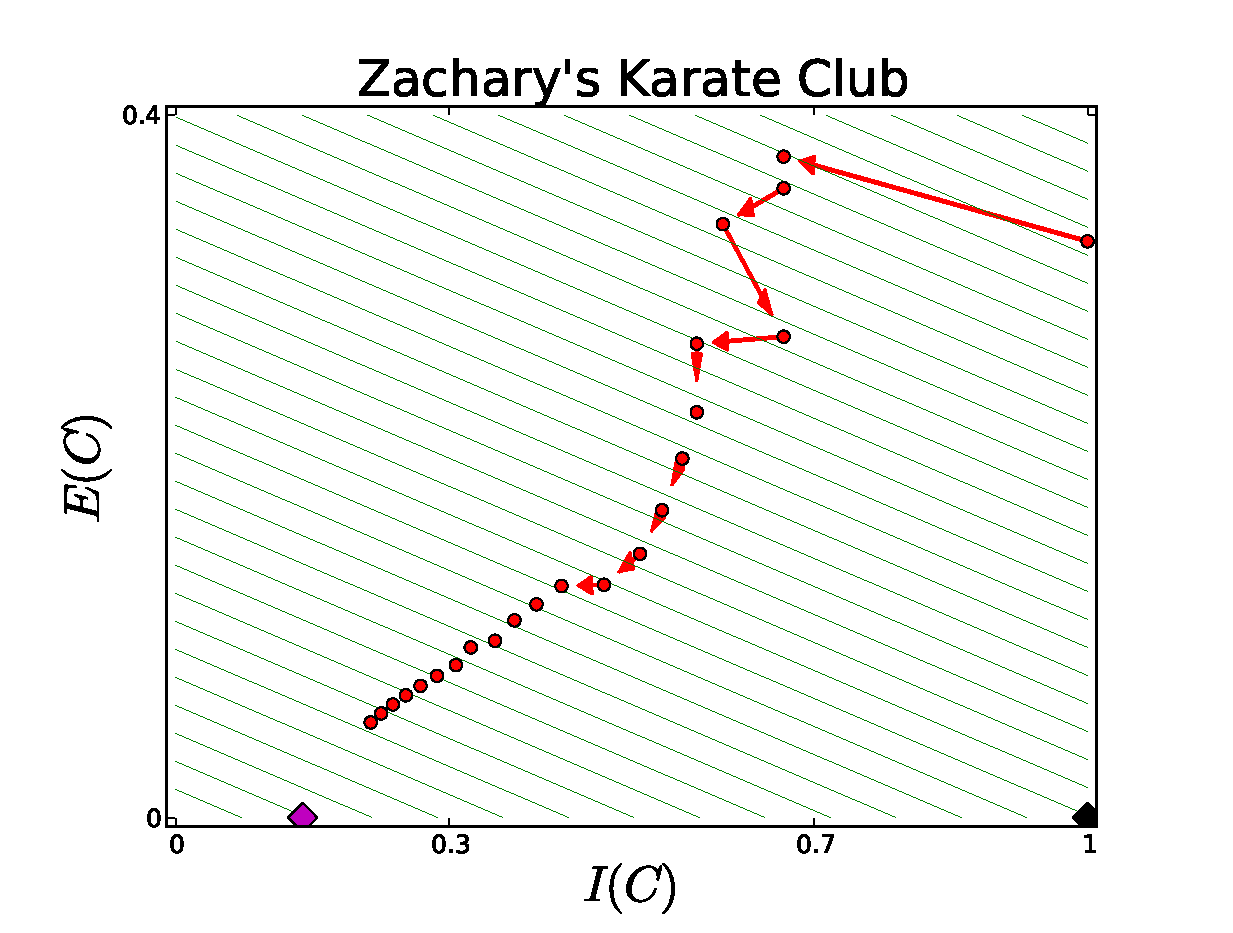
\includegraphics[width=2.8in]{Figures/volume_karate}
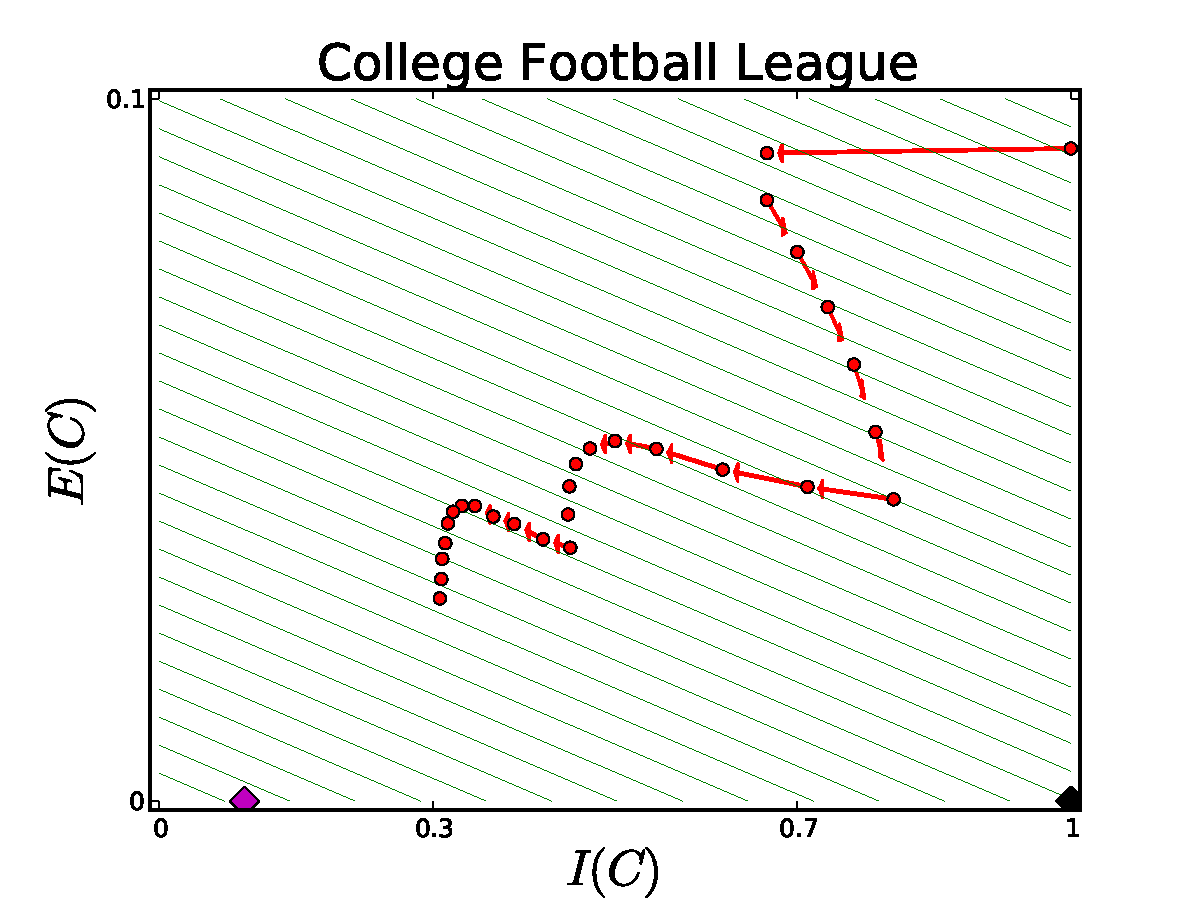
\includegraphics[width=2.8in]{Figures/volume_cfl}
\caption{Tracing of communities found by volume through the IE plane for a maximum of 100 steps. The lower left diamond is the $(I(C), E(C))$ point corresponding to a community of the entire graph.  The lower right diamond is the $(I(C), E(C))$ point corresponding to an ideal community.  The path corresponds to the intermediatory $(I, E)$ values of adding nodes that optimize the metrics using Greedy Algorithm \ref{alg_greedy_single}.}
\label{fig_real_volume}
\end{figure}

\begin{figure}[!t]
\centering
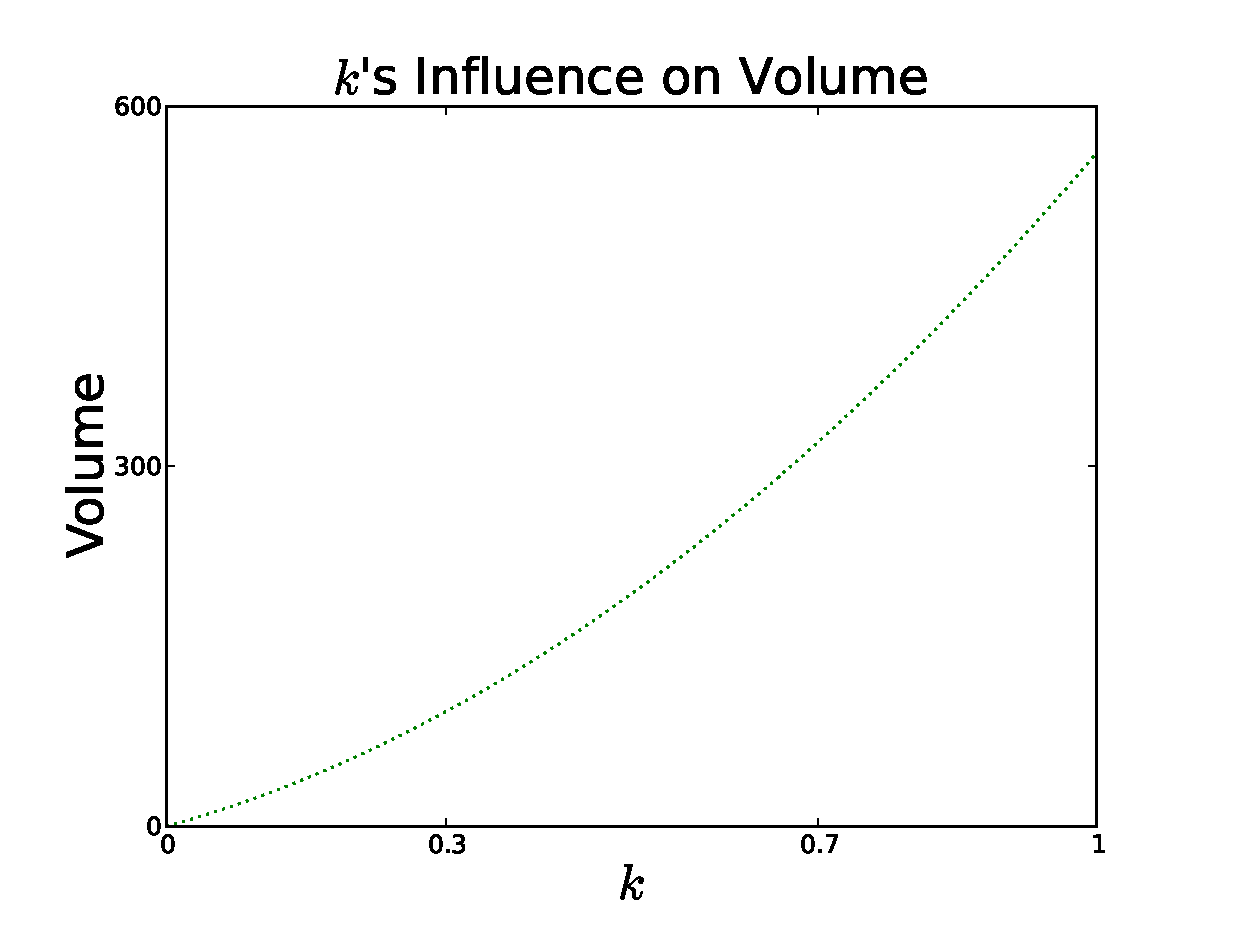
\includegraphics[width=2.8in]{Figures/volume_k}
\caption{The affect, increasing the size of the community has on volume, even for a constant $I(C)$ and $E(C)$.}
\label{fig_volume_k}
\end{figure}


% subsubsection*************************************
\subsubsection{Conductance}
For conductance the level sets are rays radiating from $(I, E) = (0, 0)$, see {\it Fig. \ref{fig_single_ls}}.  As the rays come closer to horizontal, $E(C) = 0$, conductance is closer to optimal.  Near $E(C) = 0$, changes to internal density have little effect on the value of conductance.   Improvements in conductance come from modifying the community to decrease $E(C)$ as much as possible. If the rays are away from $E(C) = 0$, then improvements to internal density have a larger impact on conductance. 

We now analyze the performance of the Greedy Algorithm \ref{alg_greedy_single} with conductance and four networks, results are displayed in Figure \ref{fig:conductance}.  In the College Football League, the greedy algorithm finds communities in the $(I, E)$ plane where improvements in $I$ and $E$ are balanced.  The final community found corresponds to our notion of a good community.  For Zarchary's Karate Club, the greedy algorithm begins to enter the region where external density determines conductance and returns a community of debateable quality.  This effect is more emphasized in the relativity and astrophysics co-author networks.  The greedy algorithm intially returns communities in the region of the $(I, E)$ plane with balanced weightings between internal and external density.  When external density reaches the region of low external density, the level sets show that small improvements to external density at the cost of lower internal density dramatically improve conductance.

This is the cause of the problem found by Leskovec et. al \cite{leskovec}.  As a metric, conductance either incorporates internal density, as in the small College Football communities, or does not incorporate internal density, as in the larger Relativity and Astrophysics Co-author communities.


\begin{figure}[!h]
\centering
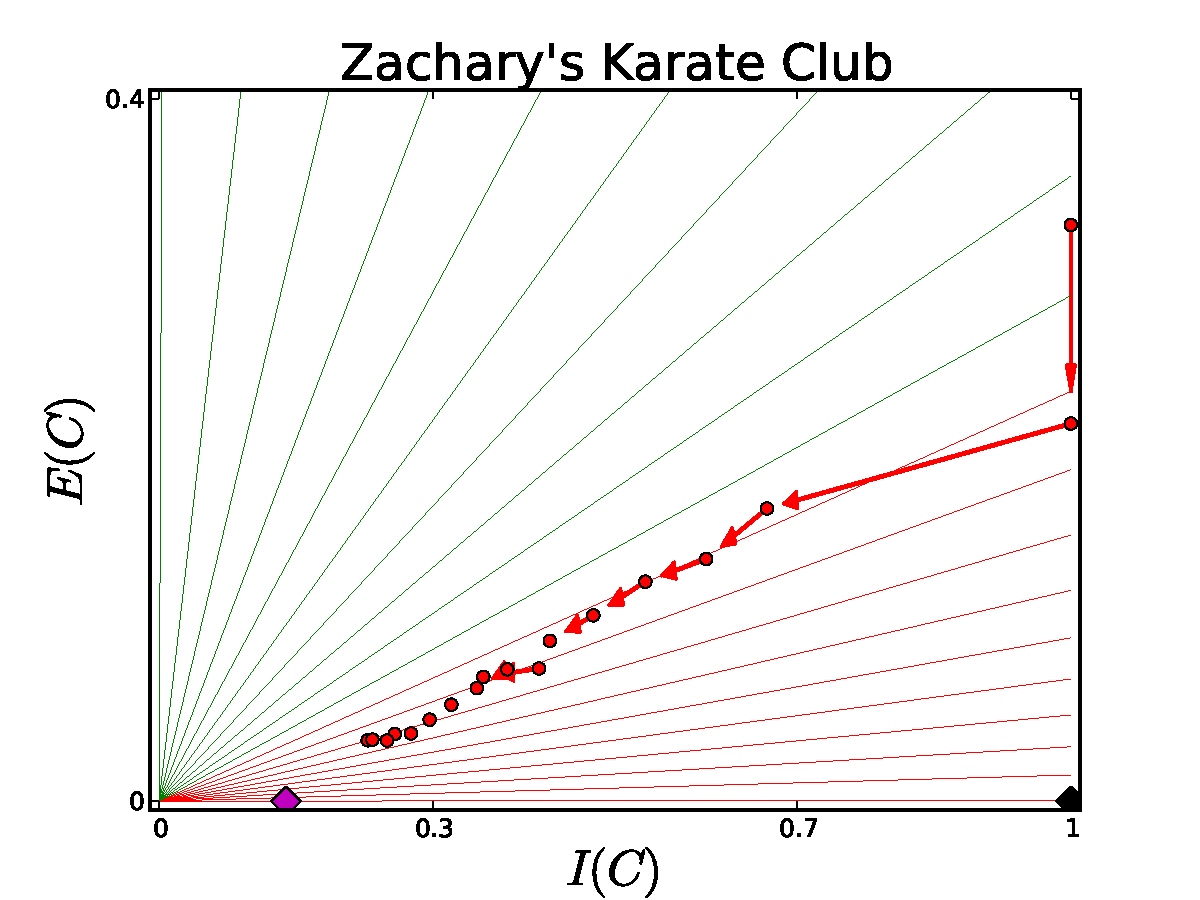
\includegraphics[width=2.8in]{Figures/conductance_karate}
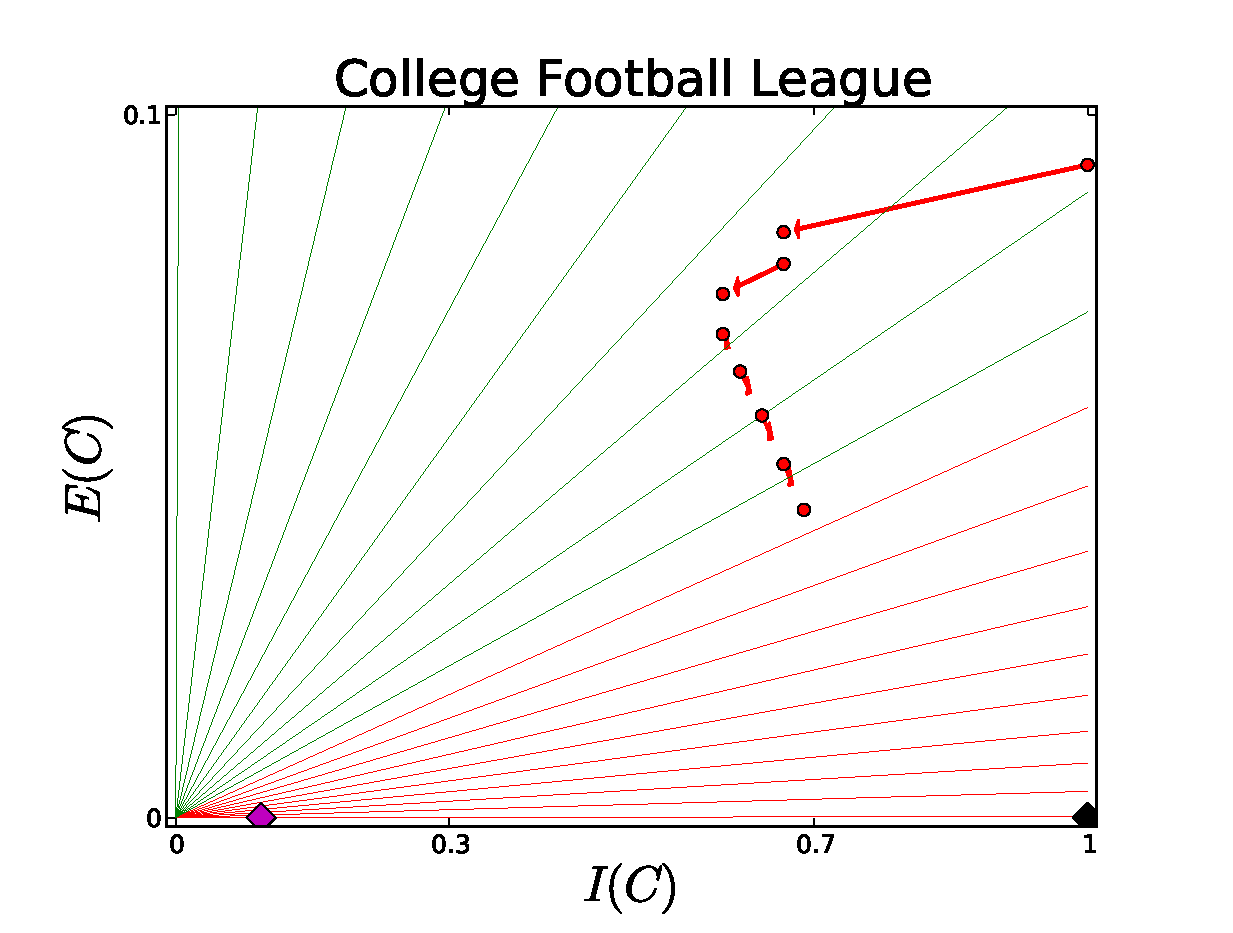
\includegraphics[width=2.8in]{Figures/conductance_cfl}
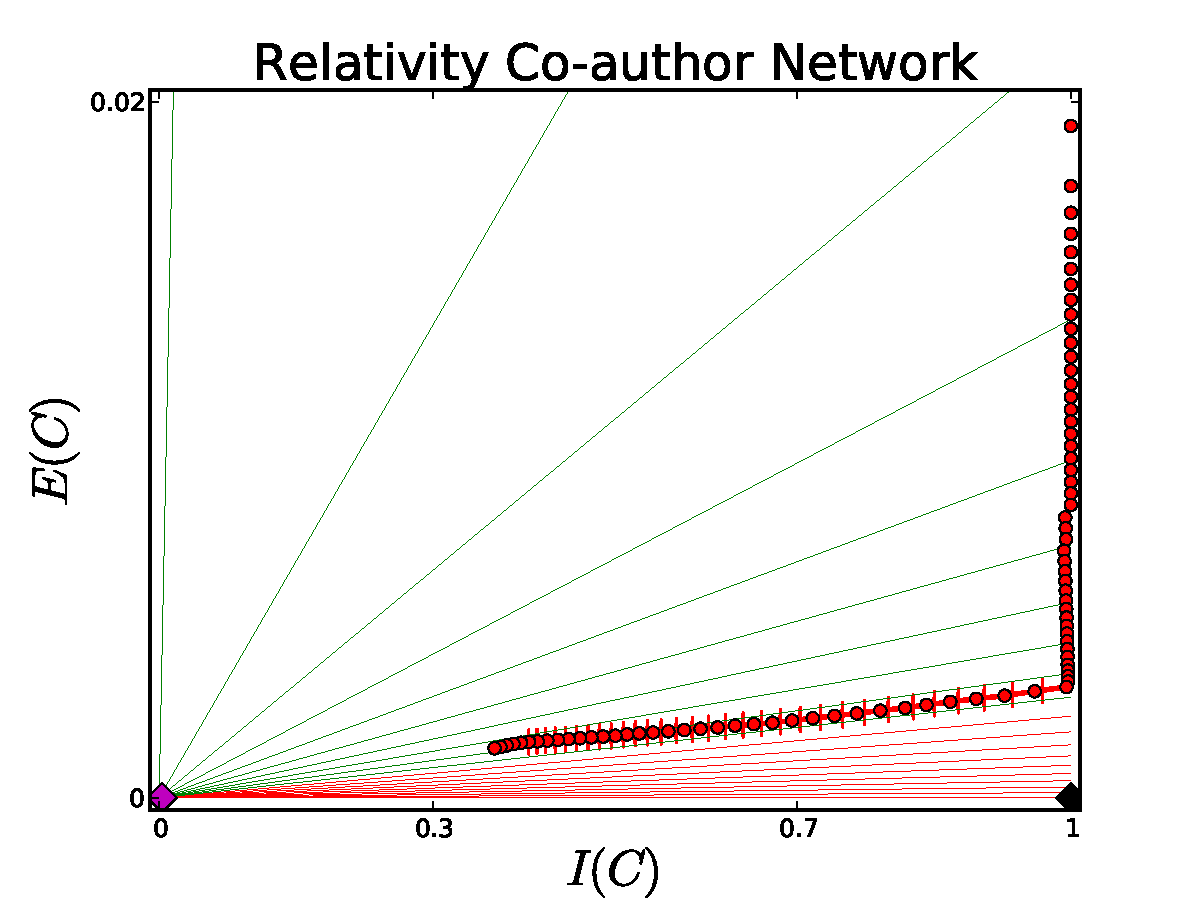
\includegraphics[width=2.8in]{Figures/conductance_relativity}
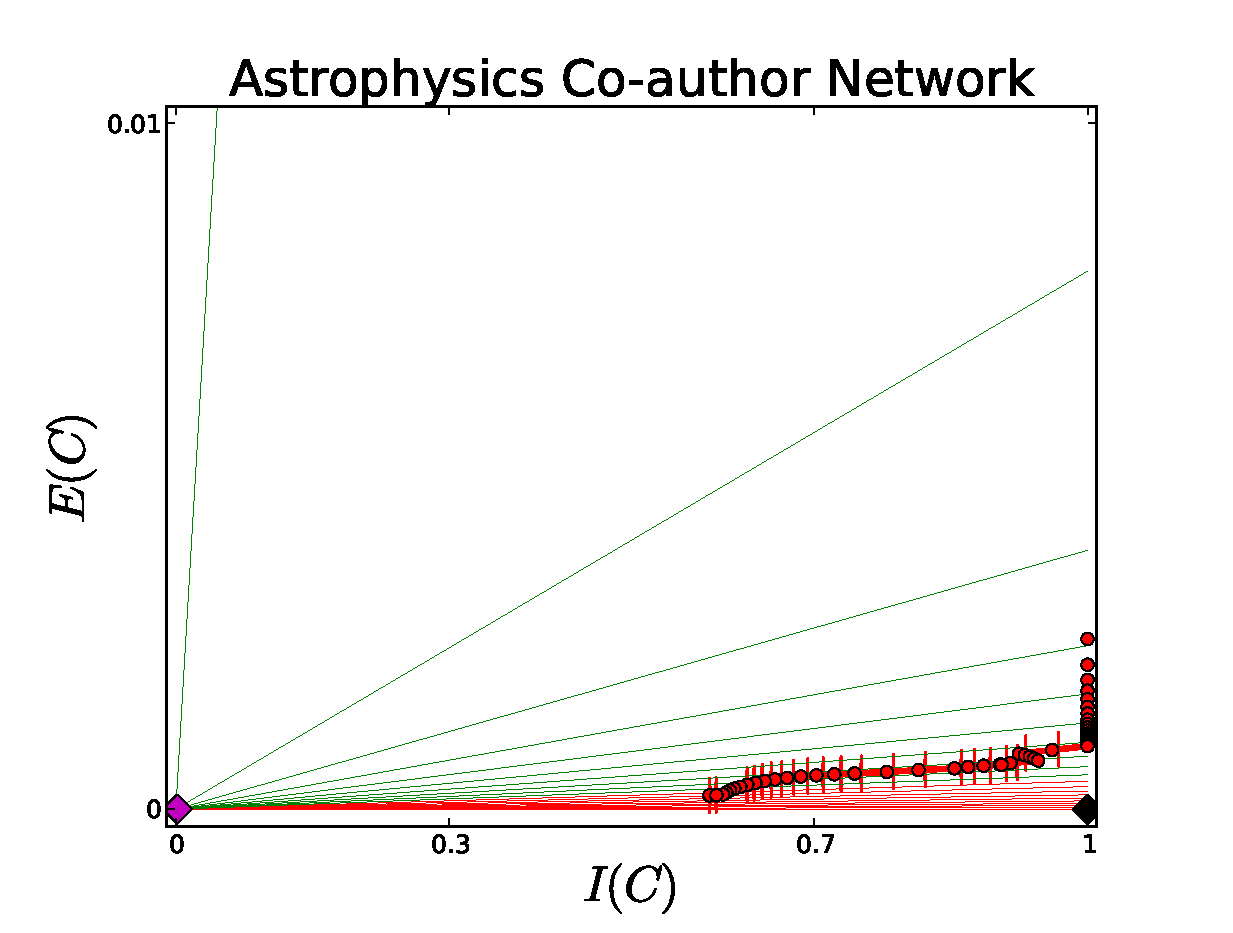
\includegraphics[width=2.8in]{Figures/conductance_astro}
\caption{The progression of communities that optimize conductance.  Note, both the entire graph and the ideal community optimize conductance.  In the relativity and astrophysics networks, we stop following the progression of conductance once it becomes clear the entire graph will be engulfed. (In the case of the college football league, a local optimum was reached, but reports an undesireable value of conductance..)}
\label{fig:conductance}
\end{figure}

This problem is amplified by the effect a community's size has on conductance.  Now we fix the $I, E$ ratio and observe how changes in $|C| = k |V|$ affect conductance, see Figure \ref{fig:k_conductance}.  Conductance always values a larger community more favorably.  As long as the community is of small to moderate size and has a large $E(C)$ value, the greedy algorithm will return communities that to correspond to our intuition that an ideal community.

\begin{figure}[!h]
\centering
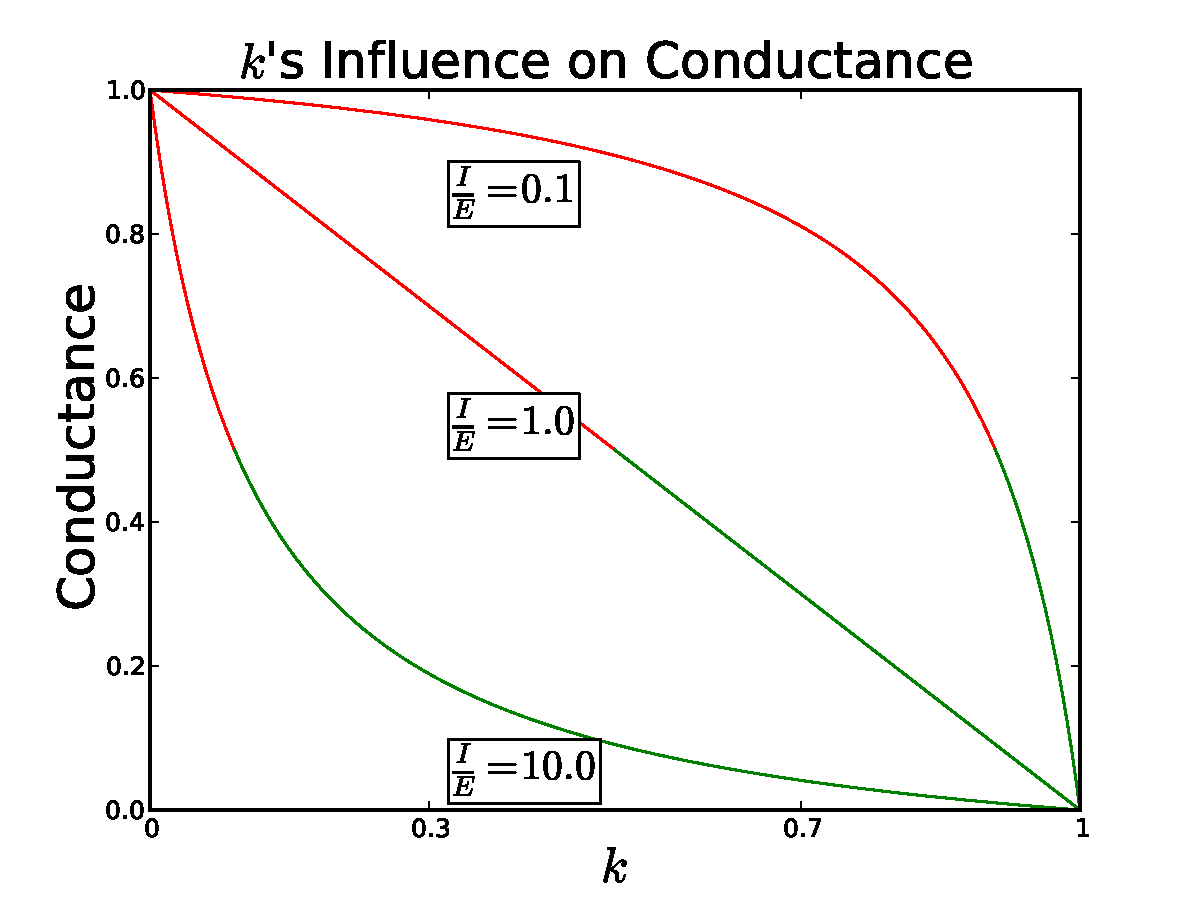
\includegraphics[width=4in]{Figures/k_influence_conductance}
\caption{Influence of size of community on the value of conductance.  The object is to minimize conductance}
\label{fig:k_conductance}
\end{figure}


% New Section******************************
\section{Set of Communities Based Metrics}

We now explore metrics that evaluate the strength of a set of communities, $S=\{C_1, C_2, \dots, C_n\}$.  Several community detection methods are based on finding a partitioning of the network that optmizes such a metric.  The most popular of these metrics is, modularity developed by Newman \cite{newman}.


% New Subsection **********************************************
\subsection{Internal Density, External Density, and Conciseness}

Our parameterization of internal and external density for single community metrics can not be directly applied to a set of communities, $S = \{C_1,C_2,...C_n\}$. We begin as we did for single communities and consider the characteristics of a good set of communities.  A set of good communities is a set of cliques such that every edge is within some community and every community is a maximal clique. Hence an ideal set of communities has three parameters. Internal density is a representation of how close the set of communities is to being a set of cliques. External density is a representation of how close the set of communities are to covering all edges in the graph. Size of the set of communities is a representation of how concise the set of communities are. With the same methodology for parameterizing and understanding metrics of individual communities we proceed to parameterize metrics for sets of communities with {\it internal density}, {\it external density}, and {\it conciseness}.  Formal definitions follow.

\begin{definition}[Internal Density of a Set of Communities] For a set of communities, $S = \{C_1, C_2, \dots, C_n\}$, the internal density of the set is the sum of the number of edges that do exist within each community compared to the mazimal number of edges that could exist.
\begin{equation}
I(S) = \frac{\sum_{C \in S} \left( \sum_{u \in C} \sum_{v \in C} w(u,v)\right)}{\sum_{C \in S}|C|(|C| - 1)}
\end{equation}
\label{def_int_set}
\end{definition}

\begin{definition}[External Density of a Set of Communities] In a set of communities, $S$, the {\sc Ext\_Edges} is the set of edges not covered by any community.  External density is the number of edges in {\sc Ext\_Edges} compared to the number of edges in the graph.
\begin{equation}
E(S) = \frac{\sum_{(u, v) \in \mbox{\sc Ext\_Edges}} w(u,v)} {\sum_{u,v \in V}w(u,v)}
\end{equation}
\label{def_ext_set}
\end{definition}

\begin{definition}[Conciseness of a Set of Communities]  Conciseness is the size of $S$.
\begin{equation}
\mbox{\sc Conciseness}(S) = |S|
\end{equation}
\label{def_conciseness}
\end{definition}

Our choice of defining the parameters, allows the analysis of any set of communities, including overlapping communities.  In particular, our definition of internal density for a set of communities, allows nodes to be placed in multiple communities.  External density is independent of overlapping communities, as well as conciseness.

\begin{definition}[Ideal Set of Communities]
A set of communities, $S$, is ideal if it is a set of maximal cliques that cover the graph in very few communities:
\begin{eqnarray*}
I(S) &=& 1\\
 E(S) &=& 0 \\
|S| &=& \mbox{number of connected components of the network.}
\end{eqnarray*}
\end{definition}

All three parameters are necessary to ensure a complete description of a set of communities.  For any two parameters, there exists a set of communities that can optimize those two parameters.  Failure to evaluate the third parameter reveals an undesired characteristic of the set of communities. Figure \ref{fig_corner_sets}, illustrates the types of communities that can optimize for any two parameters.

\begin{figure}[!h]
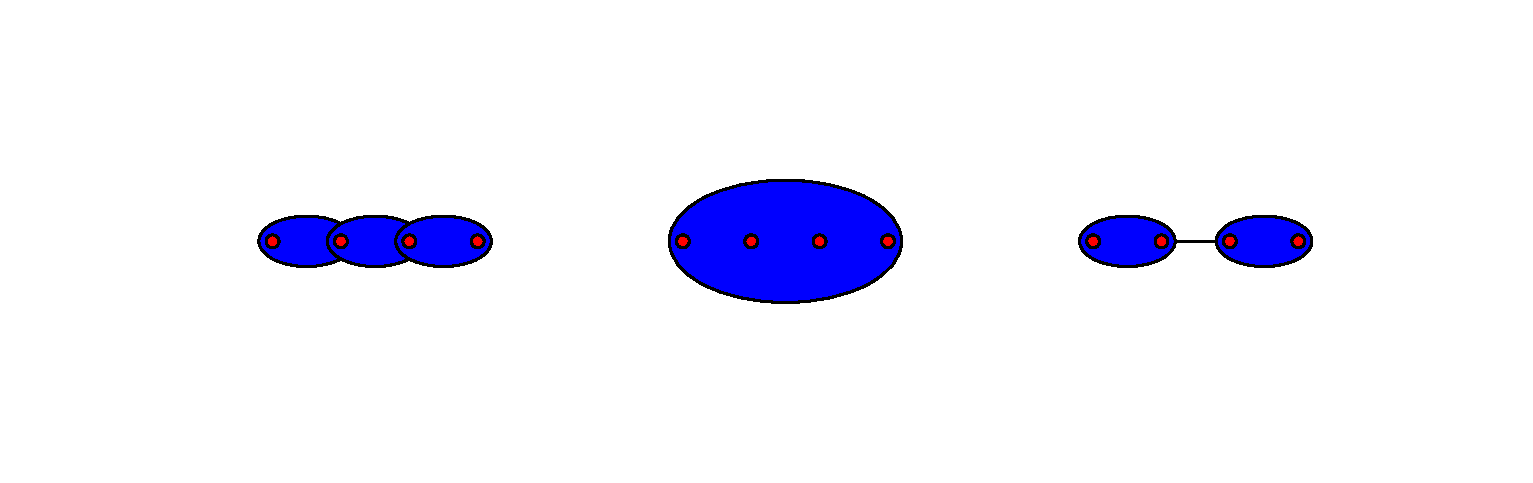
\includegraphics[width=6in]{Figures/pathological_graphs}
\caption{The communities that optimize $2$ out of $3$ parameters.  Nodes are in red, lines are edges, and communities are blue ellipses.  The left community configuration optimizes $I(S) = 1$ and $E(S) = 0$, but not conciseness at $|S| = 3$.  The middle configuration optimizes $E(S) = 0$, $|S| = 1$, but not internal density at $I(S) = \frac{1}{2}$.  The right configuration optimizes $I(S) = 1$ and conciseness at $|S| = 1$, but does not optimize external density at $E(S) = 1$}
\label{fig_corner_sets}
\end{figure}

% New subsection********************
\subsection{Study of Relevant Metrics}

Modularity is the most popular of these metrics.  It compares the number of internal edges found, to the number of expected edges in a random graph.  Modularity was developed by Newman in \cite{newman} and has found wide spread use due to the fast algorithms for maximizing modularity.  In particular, the use of dendograms in the Louvain Algorithm \cite{blondel} runs in minutes for large networks.

There is not a closed form parameterization of modularity in terms of our definitions of $I(S)$, $E(S)$, and $|S|$.  However, for each module's contribution there is a closed form parameterization in terms of internal and external density for a single community, $I(C)$ and $E(C)$.  If we allow, $p=\frac{|C|(|C|-1)}{2L}$ and $q=\frac{|C|(|V|-|C|)}{2 L}$, where $L$ is the number of edges in the graph then:
\begin{equation}
 \mbox{\sc Modularity}(S) = \sum_{C \in S} p I(C) - \left(p I(C) + q E(C)\right)^2.
\end{equation}

We first note that if there exists a set of disjoint cliques in the graph, only a partitioning of each clique into a module maximizes modularity.  Modularity already aligns more strongly with our understanding of strong communities than previous metrics.  

\begin{figure}[!h]
\centering
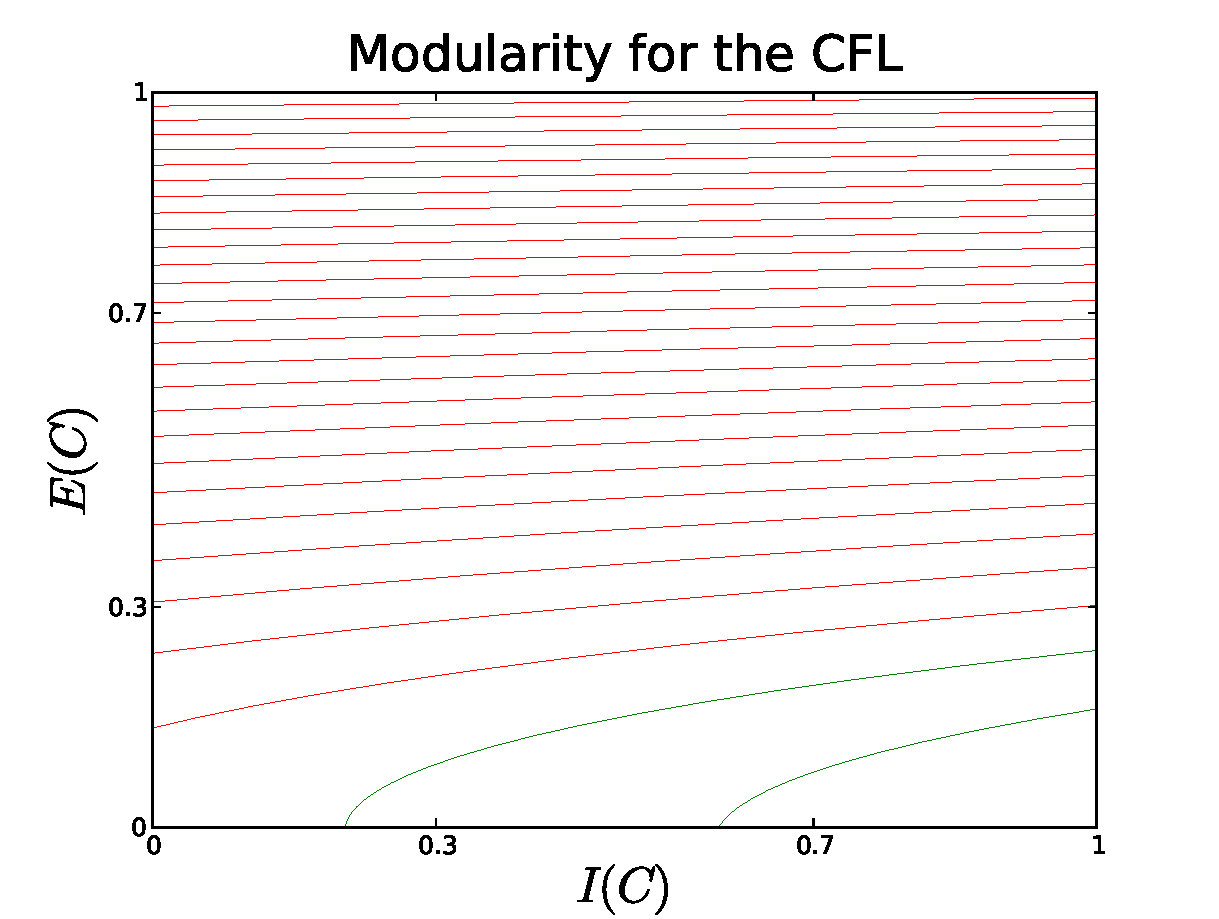
\includegraphics[width=3in]{Figures/cfl_mod_ls}
\caption{The level sets of how {\sc Modularity} treats the $I(C)$, $E(C)$ space for one community of size 9 in the CFL.  Note the sharp transition from a region that heavily favors improvements in external density to a region that heavily favors improvements in internal density($E(C) < 0.1$).}
\label{fig:mod_ls}
\end{figure}

We can not plot the level sets for modularity over a set of communities, but we can plot the level sets for the contribution to modularity from each community.  In Figure \ref{fig:mod_ls} we find that modularity is a two part optimization.  When $E(C)$ is large, modularity maximization attempts to decrease $E(C)$ as quickly as posisble.  Once a threshold of $E(C)$ is crossed, modularity maximization attempts to increase $I(C)$ as quickly as posisble.  The transition between these two phases of optimization is sudden and revealed by a dramatic turn in  the level set curves.  The larger the graph the more sudden this transition.

\begin{figure}[!h]
\centering
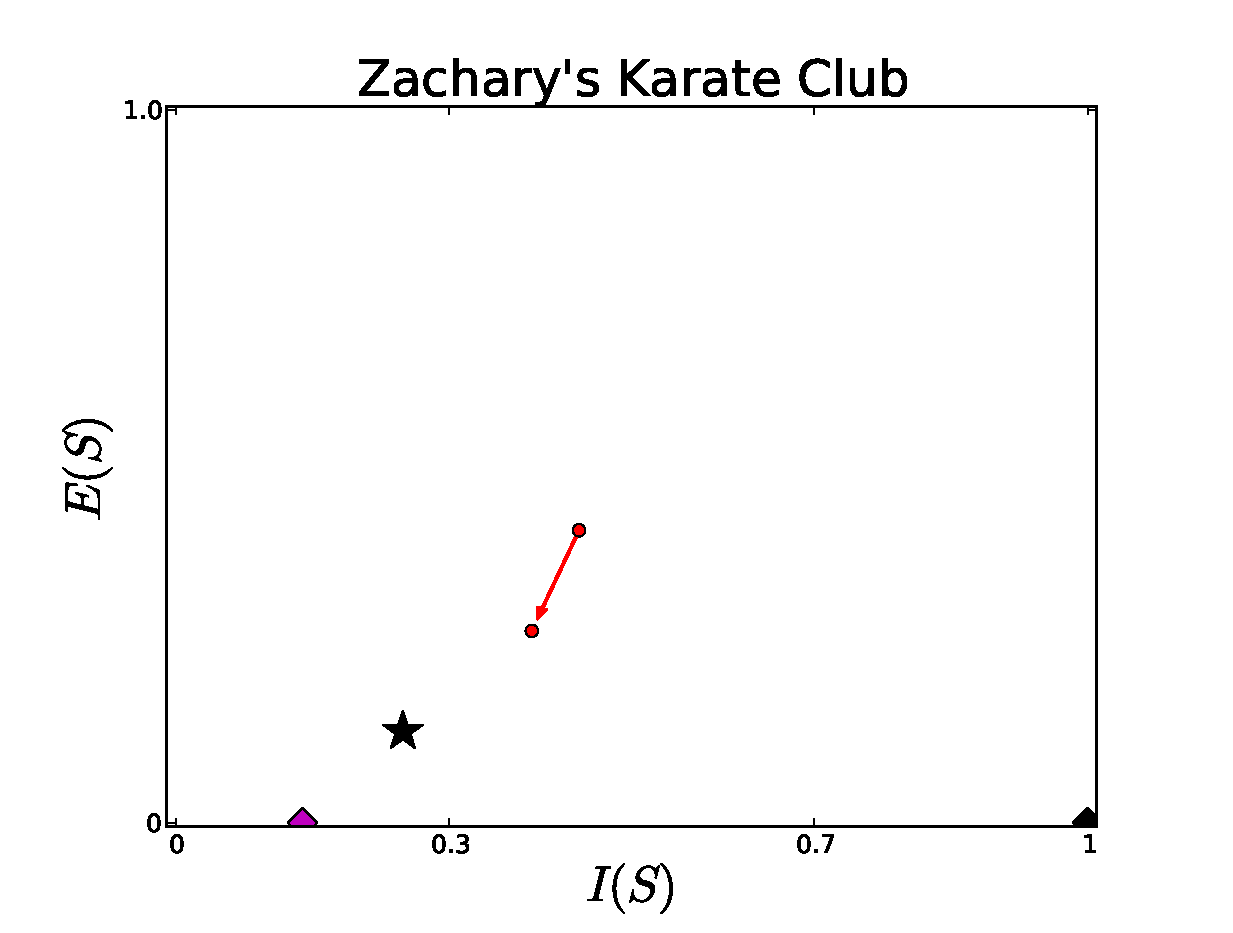
\includegraphics[width=2.8in]{Figures/modularity_karate_sets}
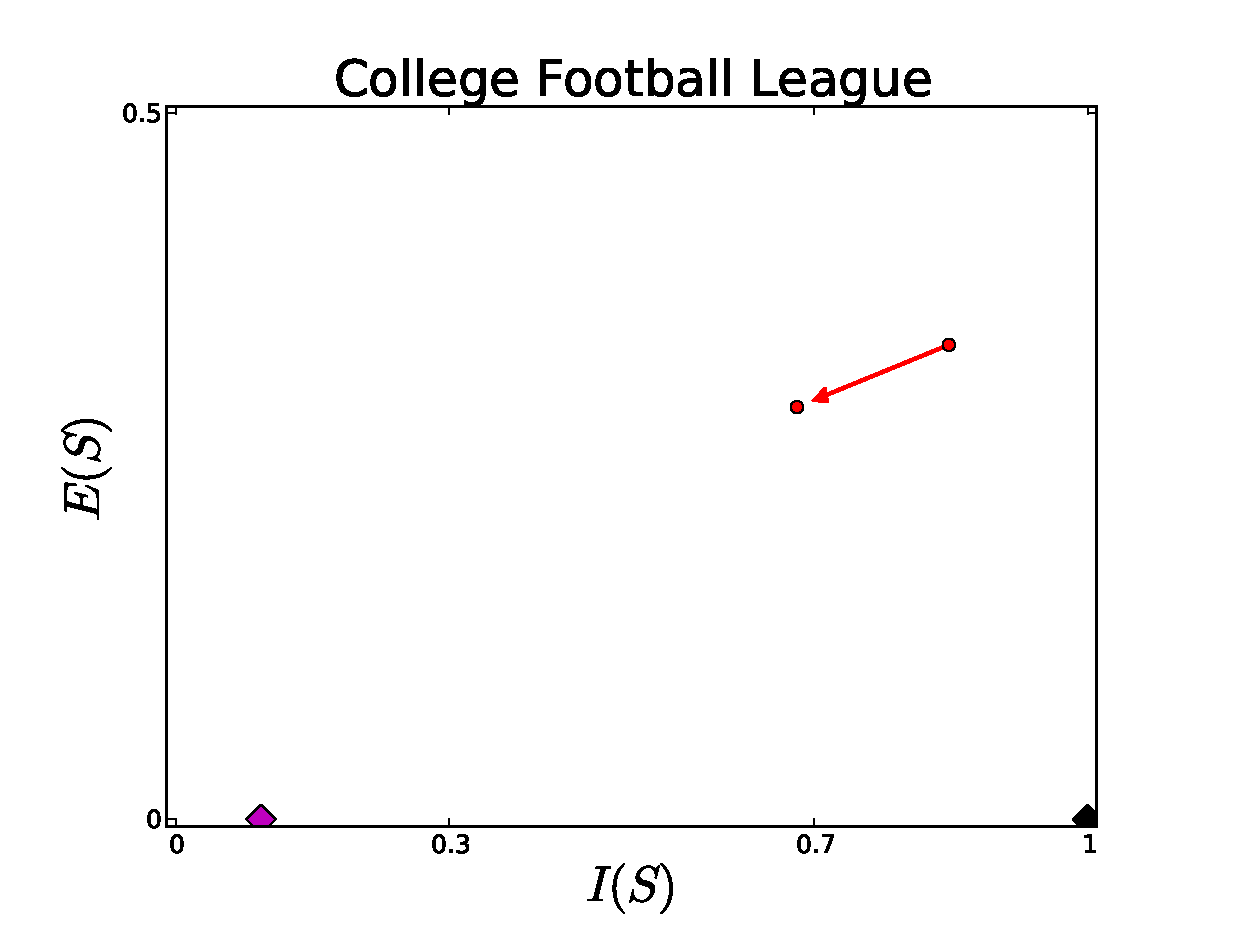
\includegraphics[width=2.8in]{Figures/modularity_cfl_sets}
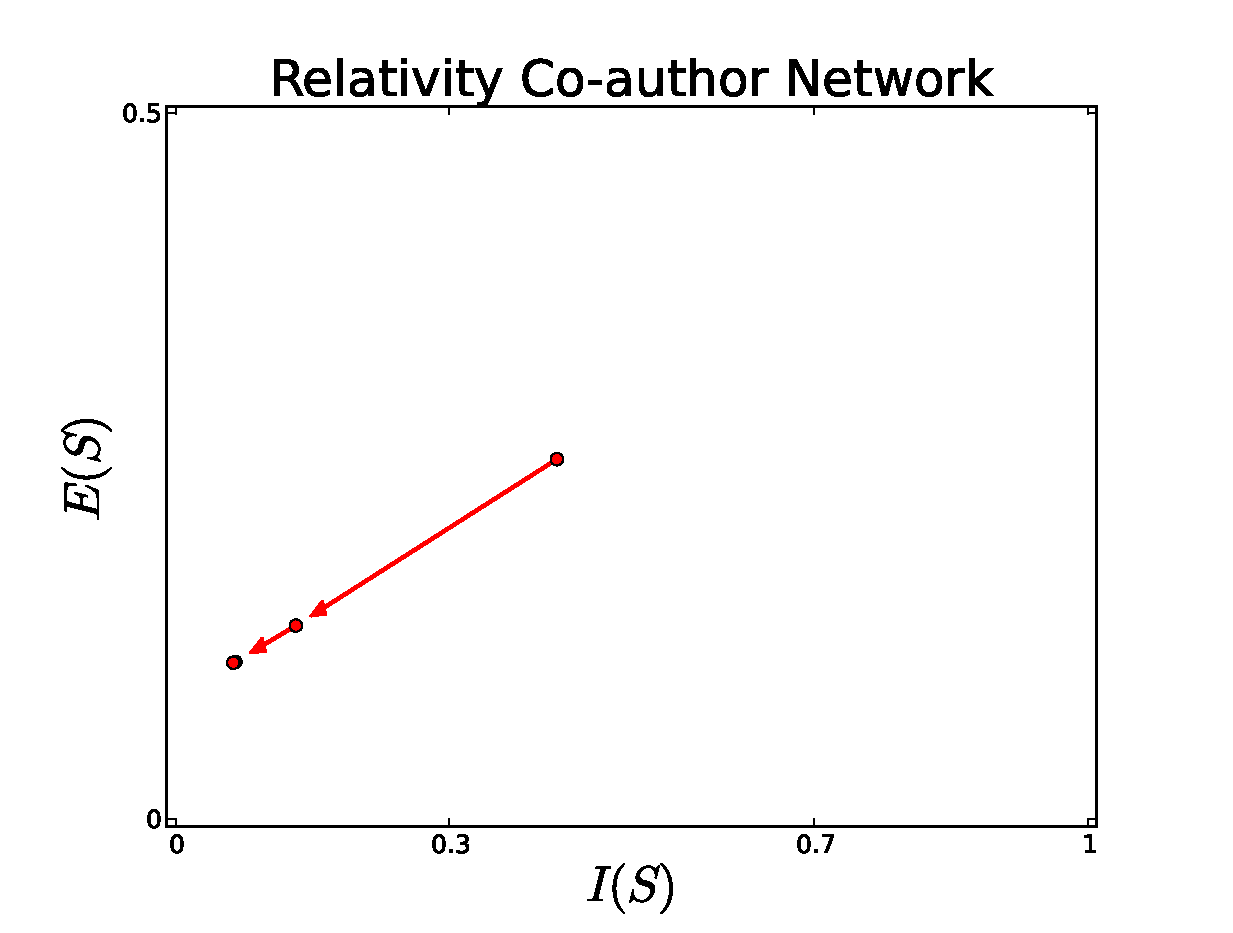
\includegraphics[width=2.8in]{Figures/modularity_relativity_sets}
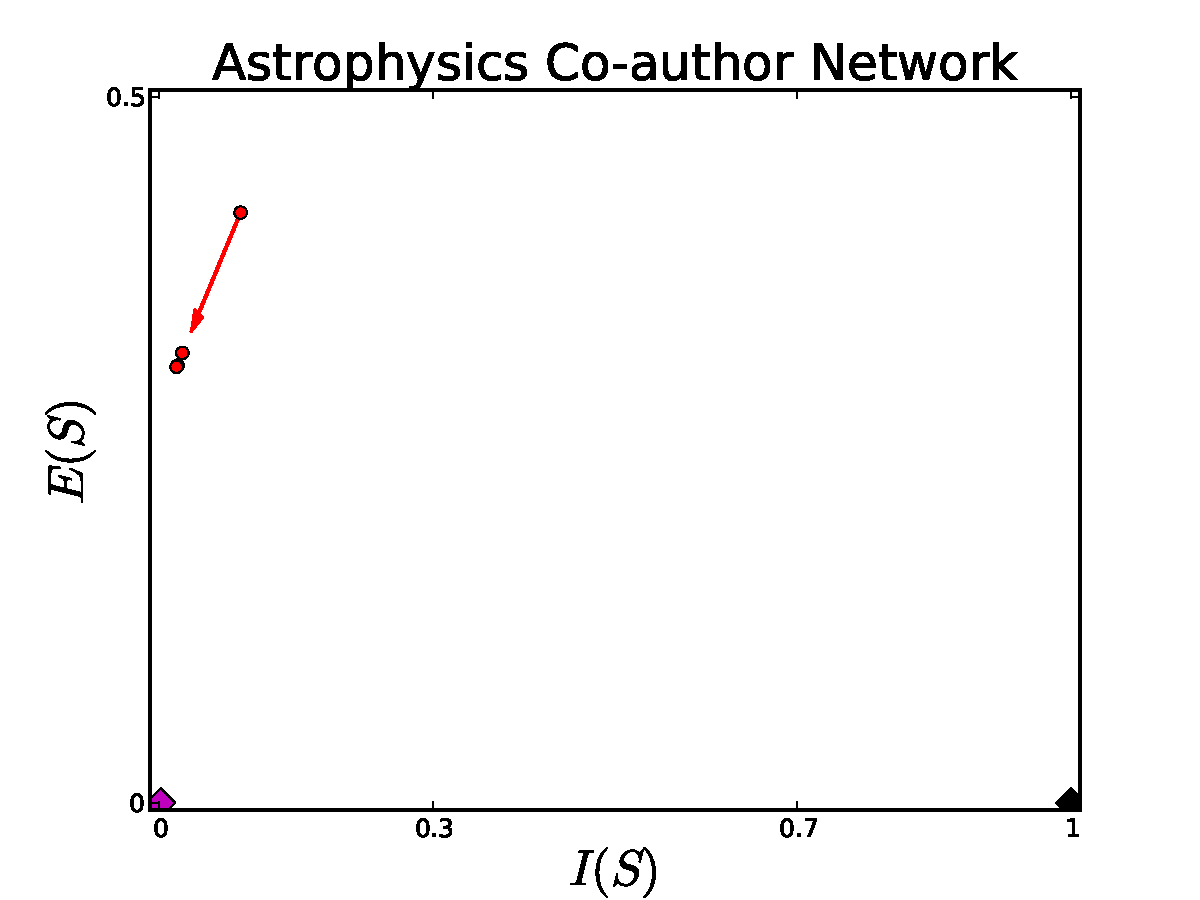
\includegraphics[width=2.8in]{Figures/modularity_astro_sets}
\caption{Here we run the Louvain Algorithm \cite{blondel} to maximize modularity.  The $(I(S), E(S))$ path is each level of the dendogram. The $(I(G), E(G))$ value for the entire graph is the diamond in the lower left.  In the general relativity and astrophysics co-author networks, modularity does not present much of an improvement over $I(G)$ and has a much higher $E(G)$ value.}
\label{fig_real_mod_sets}
\end{figure}


JTODO They say modularity has a resolution limit, but that is just because modularity at first tries to optimize external density which is prone to joining communities together. \cite{JTODO}






% New Chapter *****************
\chapter{A New Metric: Linearity}

Previously analyzed metrics fell into two categories.  In the first, the metrics: edges cut, cut, ratio, expansion, and internal density, reflect either internal or external density but not both.  These metrics are optimized by sets of nodes that do not provide insite into the structure of the network.  The second category, including modularity and conductance, is unpredictable.  They have the same values for radically different communities.  In being unpredictable, conductance and modularity, sometimes produce strong communities and sometimes, especially as the size of the communities increases, return poorly connected communities\cite{JTODO}.

In this chapter we will present metrics for single communities and sets of communities that measure both internal and external density and are consistent.


% new section************************
\section{Single Community Detection}

Let us now discuss the criteria of a good metric and find a such a metric.  In the previous chapter, we show that internal and external density provide bounds for the characteristics of diameter, average shortest path, etc.  While it is possible to design a metric that covers an arbitrary number of characteristics, we argue a metric that reflects both internal and external density provides a good measure of many characteristics.  Then, a good metric should reflect a community's internal and external density.  In particular, the metric should be optimized by the ideal community and minimized, or minimal, for communities with poor values of internal and external density.  It easy to check the how a metric handles extreme communities, but we also want an element of predictability for how the metric handles all communities.  Here is one definition of predictability.  Let communities $C$ and $C'$ have internal and external values: $(I(C), E(C)) = (x,y)$ and $(I(C'), E(C')) = (x + \delta_x, y + \delta_y)$.  Then, a metric $M$ as function of internal and external density is predictable if:
 \begin{equation}
M(x+\delta_I, y + \delta_E) - M(x,y) = M(\delta_I, \delta_E).
\end{equation}
A linear metric satisfies all mentioned criteria.
\begin{definition}[Linearity] Let $C$ be a community, {\sc Linearity}$(C)$ is a metric with a linear weighting of internal density, $I(C)$, and external density, $E(C)$.  Such that {\sc Linearity}$: C \rightarrow [-1, 1]$.
  \begin{equation}
   \mbox{\sc Linearity} (C) = a I(C) - b E(C)
  \end{equation}
The constants $a$ and $b$ are restricted to $a, b \in (0,1]$.
\end{definition}

\begin{figure}[!h]
\centering
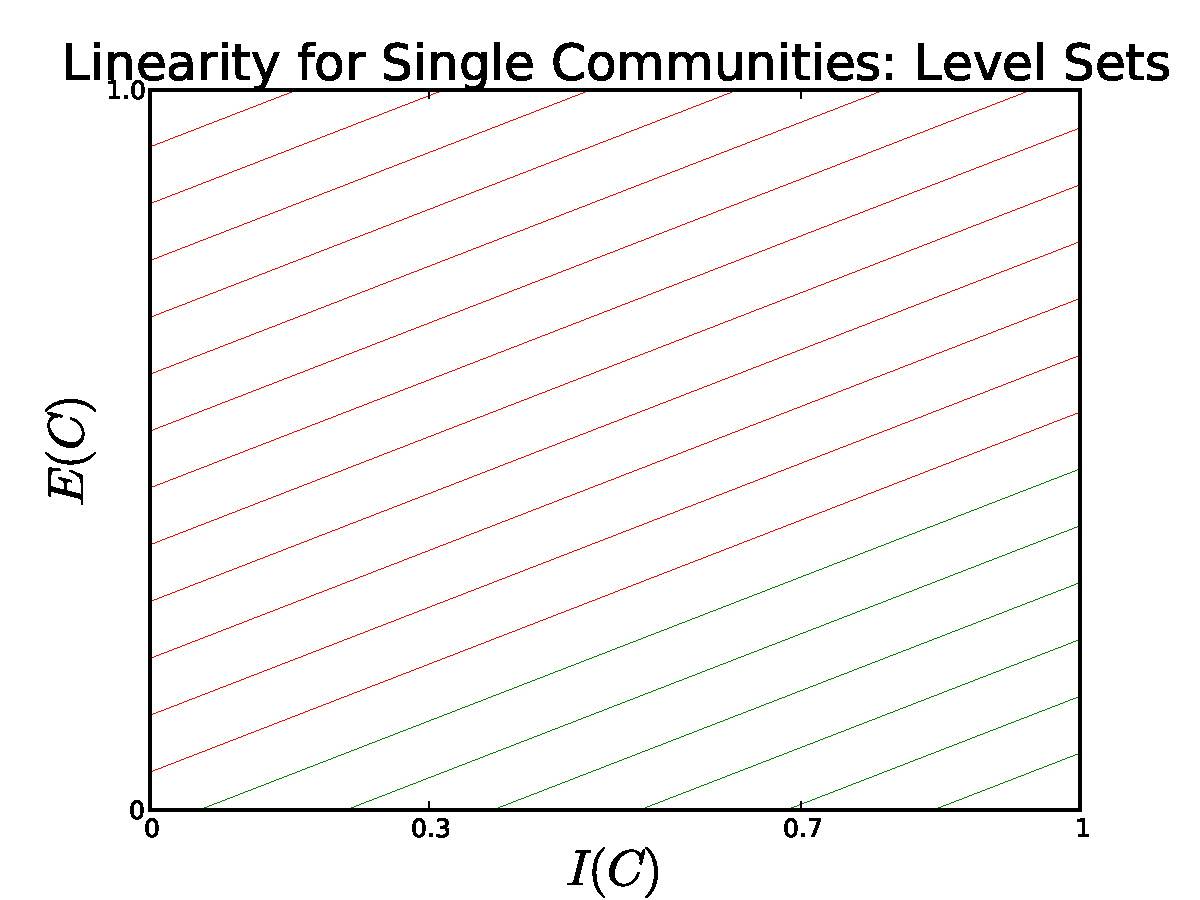
\includegraphics[width=2.8in]{Figures/linear_single_ls}
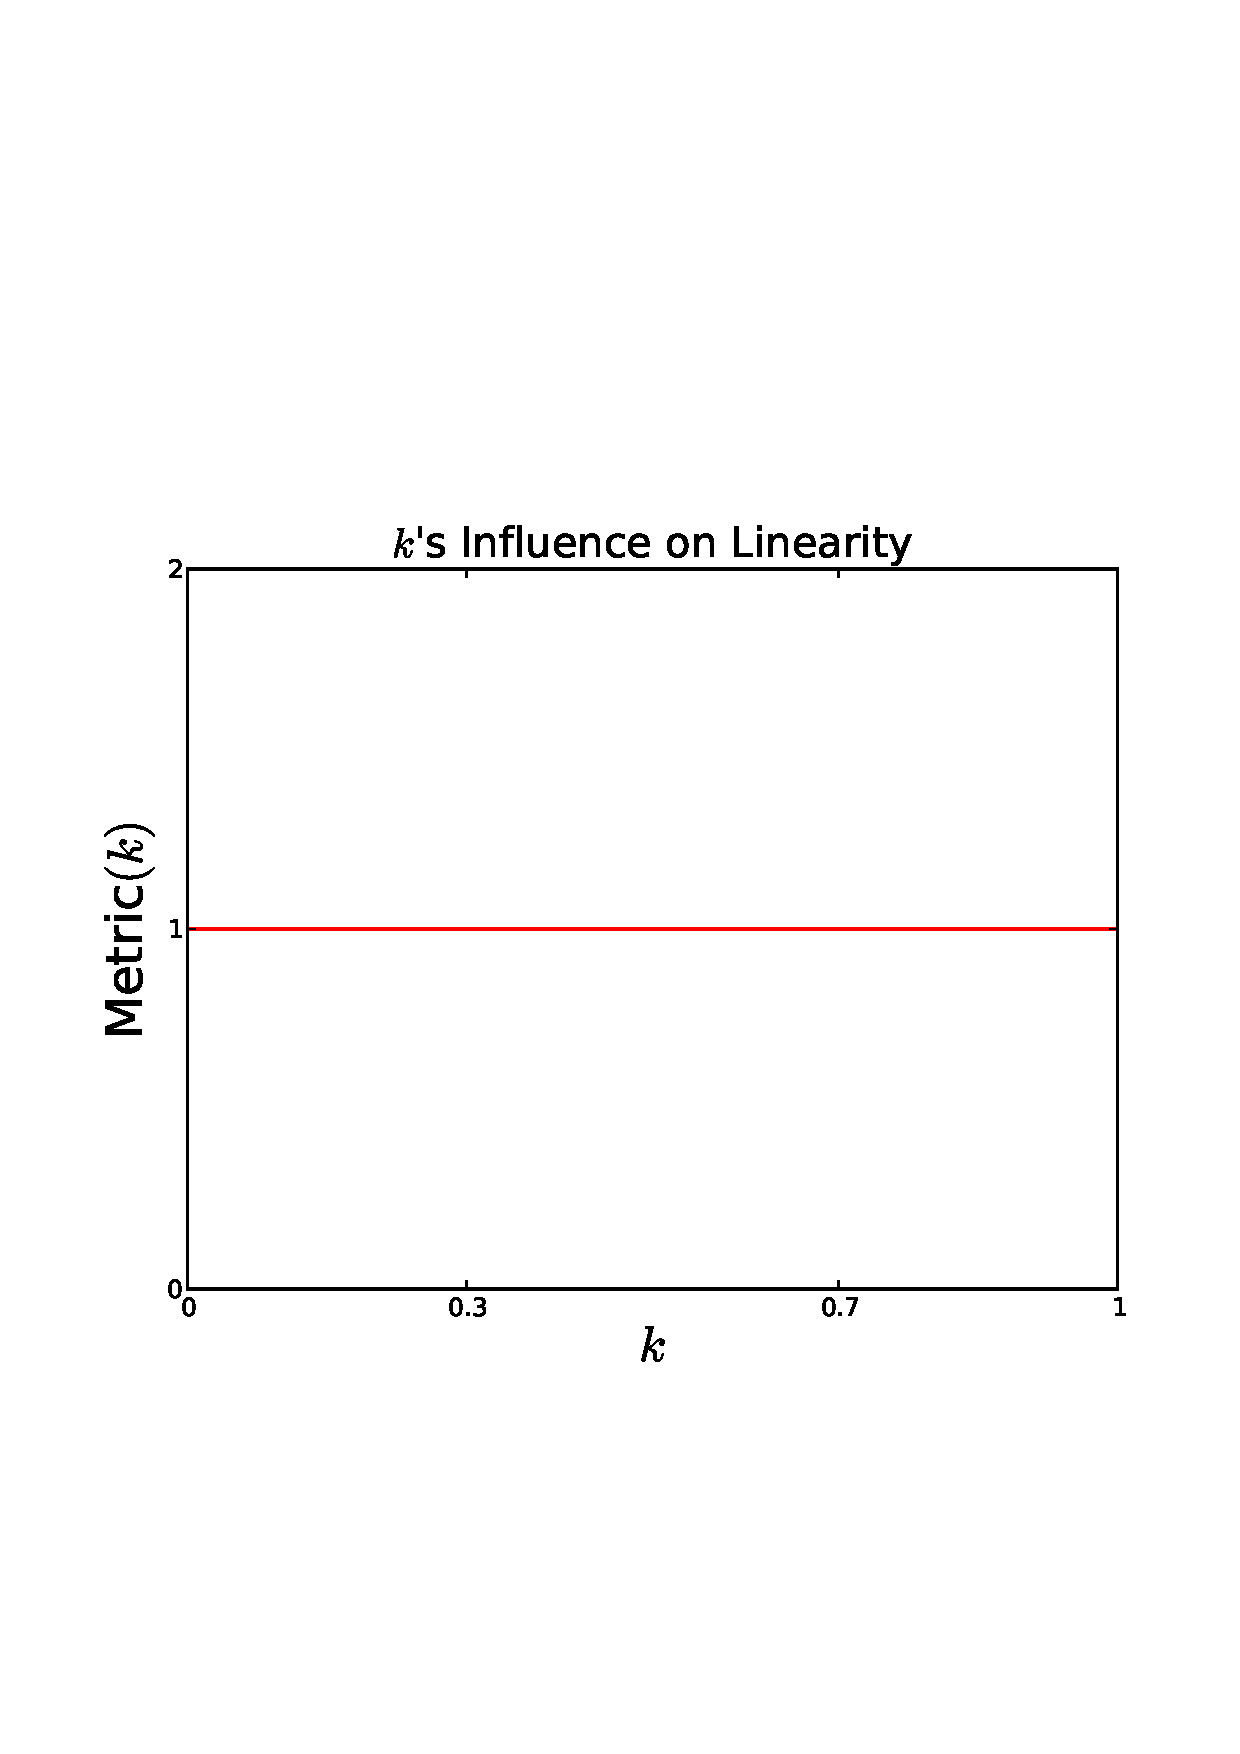
\includegraphics[width=2.8in]{Figures/linear_single_k}
\caption{The level sets are predictable.  The size of a community does not influence {\sc Linearity}.}
\label{fig:linear_single_ls_k}
\end{figure}

In some applications, we may want to relax the predictability constraint to find communities of a certain size, internal, or external density.  If this is the case, we suggest a polynomial approach to building a metric.
\begin{definition}[General Metric] The general metric for evaluating any single community is a sum of polynomial functions on internal and external density, weighted with a function of the community's size.
  \begin{equation}
   \mbox{\sc General}(C) = \sum\limits_{i = 0} f_i(C) I(C)^i - g_i(C) E(C)^i
  \end{equation}
The functions $f_i$ and $g_i$ can be any function of the size of a community.
\end{definition}
If an instance of the general equation for an application is used, the level sets and size community impact should be analyzed for elements of unpredictability.  In particular, the local and global maximums should correspond to the desired communities, and the level sets should aid finding desired communities in a manner similar to gradients.

\begin{figure}[tb]
\centering
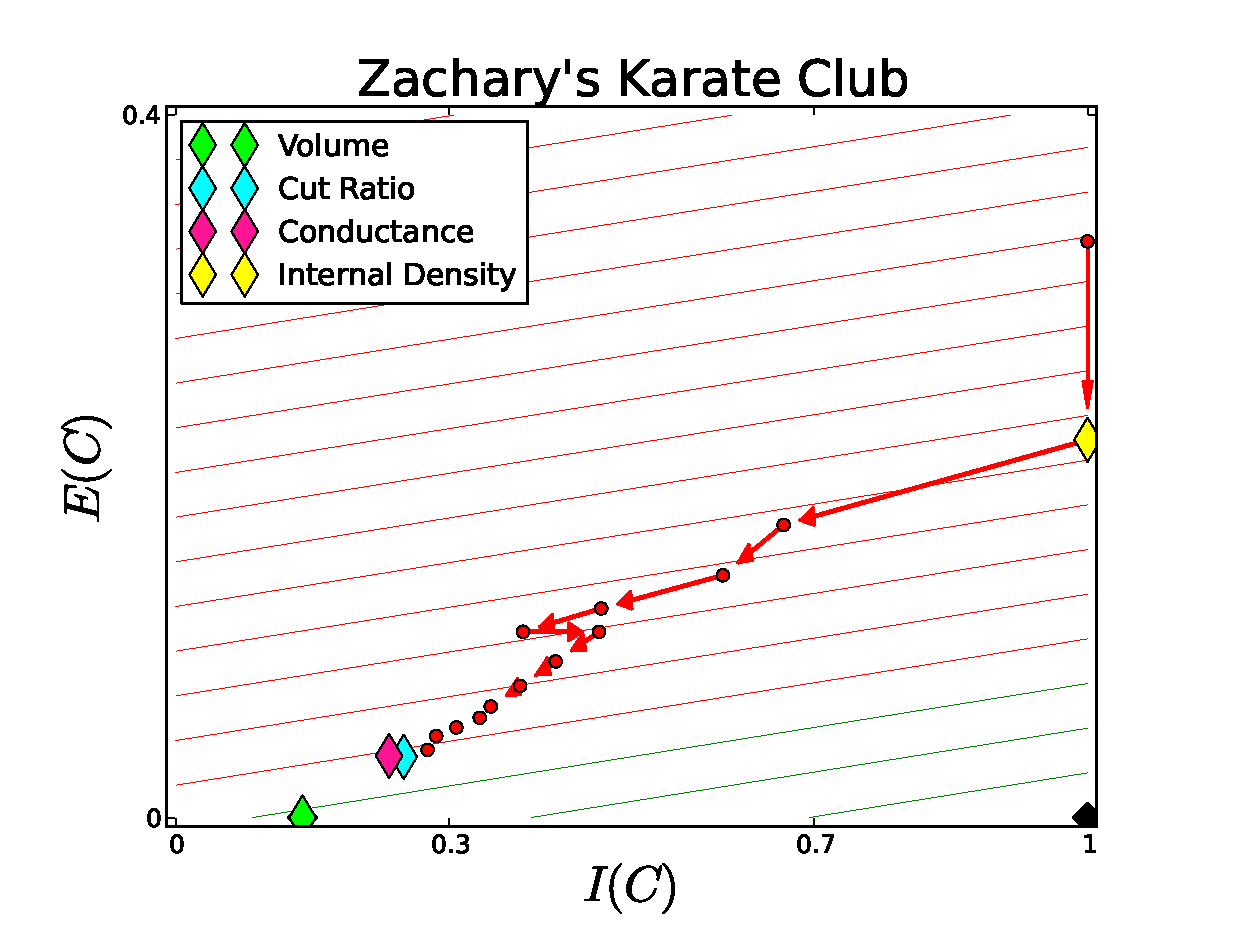
\includegraphics[width=2.8in]{Figures/linear_single_karate}
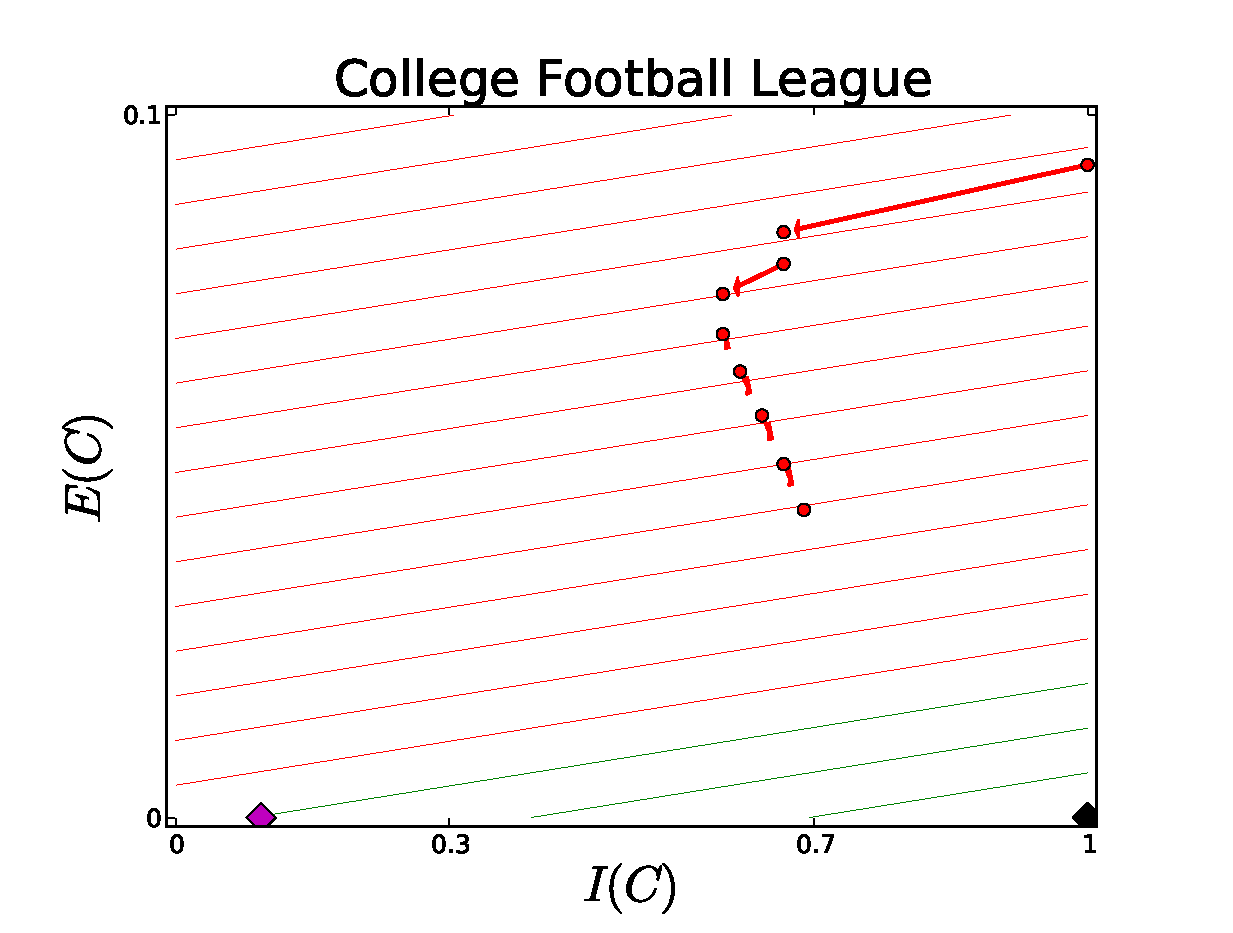
\includegraphics[width=2.8in]{Figures/linear_single_cfl}
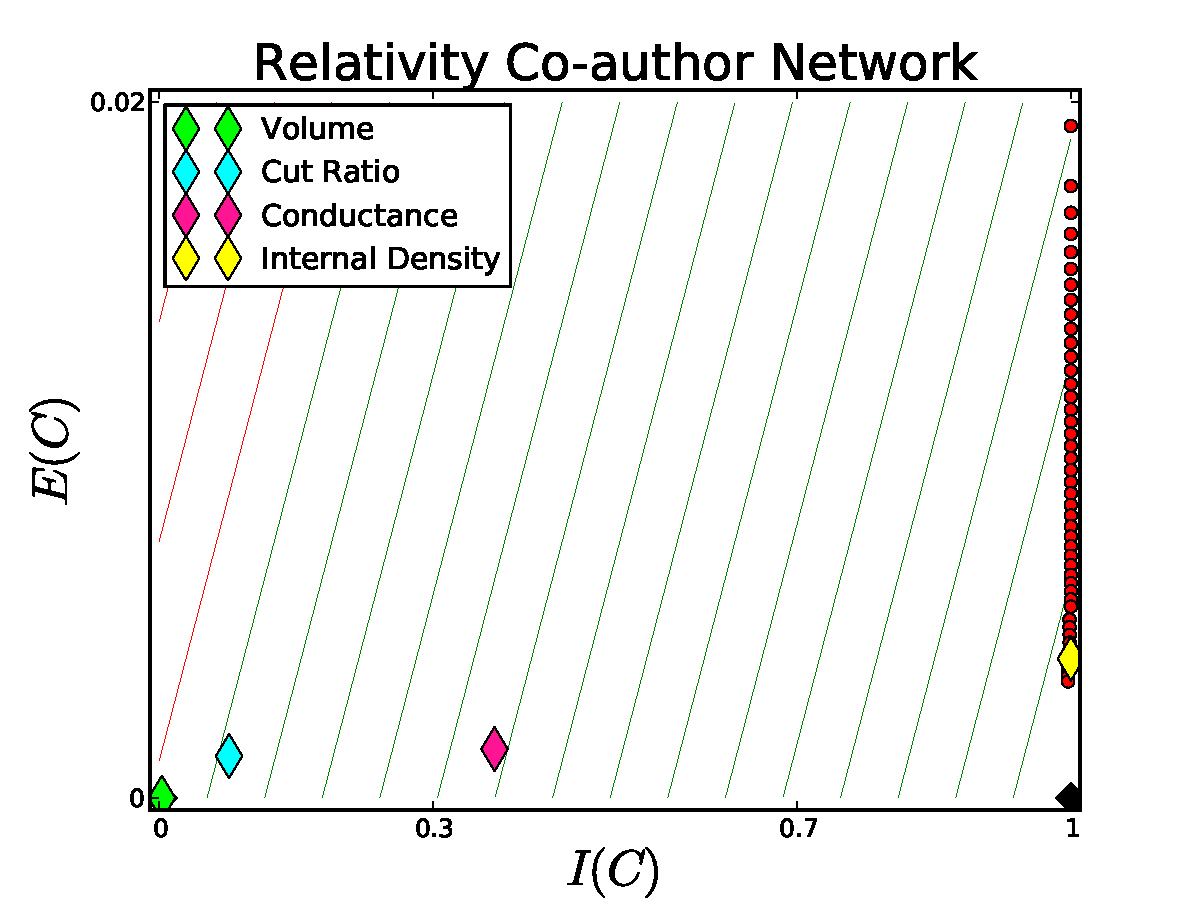
\includegraphics[width=2.8in]{Figures/linear_single_relativity}
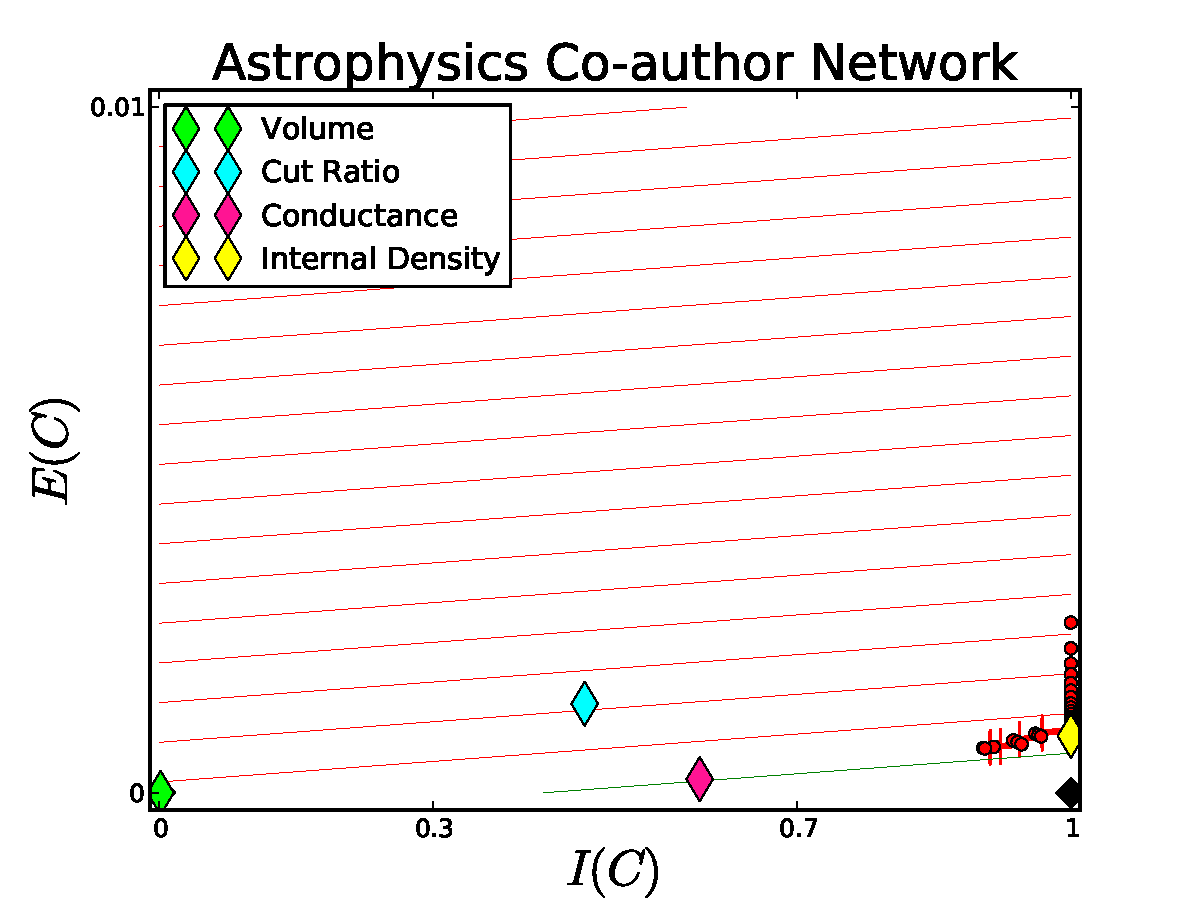
\includegraphics[width=2.8in]{Figures/linear_single_astro}
\caption{Single Communities produced by Linearity, in red.  The colored diamonds are the $(I(C), E(C))$ values produced by previously tested single community metrics.  In the Karate Club and CFL network Linearity returns a community close to conductance.  In the relativity and astrophysics network Linearity returns a community closer to internal density.  The black diamond is the ideal community, but does not exist in these networks.}
\label{fig:linear_single}
\end{figure}

We now analyze {\sc Linearity} in the same way we analyzed other single community metrics.  The level sets in Figure \ref{fig:linear_single_ls_k} reveal a predictable metric that is only optimized by the ideal community. The size of the community does not change the behavior of the metric.  We test the {\sc Linearity} metric  with the Greedy Algorithm \ref{alg_greedy_single} on four networks in Figure \ref{fig:linear_single}.  The parameters were set to $a = 1$ and $b$ required a binary search.  The parameter $b$ was set within four steps, such that the greedy algorithm did not return the entire graph or the initial community. There is room for future research on the impact of $b$.  For all possible values of $b$, we find very few different communities.





% new section *************************
\section{Multiple Community Detection}

As we constructed a linear metric for a single community, we now construct a linear metric for sets of communities, $S$.  The characteristics of a set of communities can be summarized by internal density (definition \ref{def_int_set}), external density(definition \ref{def_ext_set}) and the number of communities in the set (definition \ref{def_conciseness}).  A good metric should reflect a set of community's $E(S)$, $I(S)$, and $|S|$ values.  In particular, the metric should be optimized by the ideal set of communities and minimal for sets of communities with poor values of $E(S)$, $I(S)$, or $|S|$.  As with single community metrics, we want a predictable metric for sets of communities.  The most predictable metric is linear.
\begin{definition}[Linearity] Given a set of communities, $S = \{C_1, C_2, \dots \}$ {\sc Linearity}$(S)$ is a metric mapping $S$ to $[-2, 1]$.
  \begin{equation}
   \mbox{\sc Linearity}(S) = a I(S) - b E(S) - c |S|,
  \end{equation}
where $a,b,c \in (0, 1]$.
\end{definition}
Depending on the application, communities with particular values of internal density, external density, or size may be desired.  In these cases we recommend a polynomial expression for the metric.
\begin{definition}[General Metric]
 Our metric for single communities in its greatest generality:
  \begin{equation}
   \mbox{\sc General} (S) = \sum\limits_{i = 0} f_i(S) I(S)^i - g_i(S) E(S)^i - h_i |S|^i
  \end{equation}
\end{definition}
Whenever creating a metric of this form it is recommended to check the level sets for elements of unpredictability.

To maximize our linear algorithm for sets of communities, we will create a greedy algorithm with two stages.  The first is to use an adapted Louvain algorithm \cite{blondel} to find a partition maximizing linearity.  The final stage will be to expand each partition to include individual nodes.  This algorithm is a heuristic to maximize linearity, but runs in complexity equivalent to the Louvain Algorithm $O(JTODO)$.

We first state a conjecture about greedy algorithms.
\begin{conjecture}[Maintaining Internal Density]
Let community $C$ have internal density $I(C)$ and external density $E(C)$.  If an expansion of $C$ to include node $v_1$ results in a decrease in internal density, ie $I(C \cup v_1) < I(C)$, then expansion will only create a community with internal density $I(C \cup v_1 \cup v_2 \cup \dots \cup v_i) = I(C)$ by including a large clique, $v_1, v_2, \dots, v_i$.
\label{conj:int_density}
\end{conjecture}
We have stated the conjecture corresponding to single communities, and a similar conjecture exists for sets of communities.  The conjecture comes from our experience that once internal density is decreased it can rarely be increased by a greedy algorithm.  When internal density is decreased and then increased by a greedy algorithm a clique is involved.  Improvements to internal density are hard, improvements to external density are easy.  External density can be lowered by incorporating more nodes into the community and minimized by including the entire connected component containing the community. This leads to the development of a greedy algorithm that maintains or improves internal density, until only improvements in external density can be made.  This order of greedy algorithm is opposite the order of modularity maximization that first minimizes external density and then tries to maximize internal density, see Section \ref{JTODO}.

JTODO include pseudo code for the Louvain Algorithm

To adapt the Louvain algorithm, we must show the following property holds:
\begin{property}[Louvain Criteria]
Let $M$ be any metric, $S = \{C_1, C_2, \dots \}$, and communities $C_i$ and $C_j$ have no edges between them.  Let $S'$ be the set of communities $S$, with communities $C_i$ and $C_j$ replaced by their union, ie $S' = S - C_i - C_j + C_i \cup C_j$, then:
\begin{equation}
M(S) \geq M(S')
\end{equation}
\end{property}
The contributions of $I(S)$ and $E(S)$ decrease linearity by joining unconnected sets of nodes.  The third characteristic of our linearity metric $|S|$ can increase linearity by joining unconnected sets of nodes.  However, we will limit ourselves to $a$, $b$, and $c$ values such that overall linearity is not increased and use the Louvain Algorithm.

To adapt the Louvain algorithm, we could exchange the modularity metric for the linearity metric and get a good partition.  We take it one step further and use the Conjecture \ref{conj:int_density}.  So far we have not set the parameters $a$, $b$, and $c$ in linearity.  From the conjecture, the algorithm should optimize internal density first and then external density.  We begin with the parameters set to $a = 1$, $b = 0$, and $c = \frac{1}{ |V|}$.  Maximizing the linearity metric with these parameter values results in a partitioning of maximal cliques.  We now relax the parameter $b = \delta_b$ and complete the Louvain algorithm.  This will result in a partitioning of near cliques.  The process is continued, gradually increasing $b$ and completing the Louvain algorithm on the new parameters.  The question is when to stop increasing $b$.  In practice we increase $b$ until the partitioning of the graph is the entire graph and then retract $b$ by one increment.

JTODO include demonstration of increasing $b$.




The final step of our algorithm for maximizing linearity uses the advantage of overlapping communities.  Given the partitions produced by the previous step we augment each partition by nodes that increase linearity.  Note, because the partition produced in the previous step was a local maximal partitioning, no partition will be augmented to include another partition.

We now run our algorithm on four data sets and compare to known results and modularity results.  The object is to provide a preliminary analysis of the algorithm.  In depth results are provided in Chapter \ref{ch:datasets}.


\begin{figure}[!h]
\centering
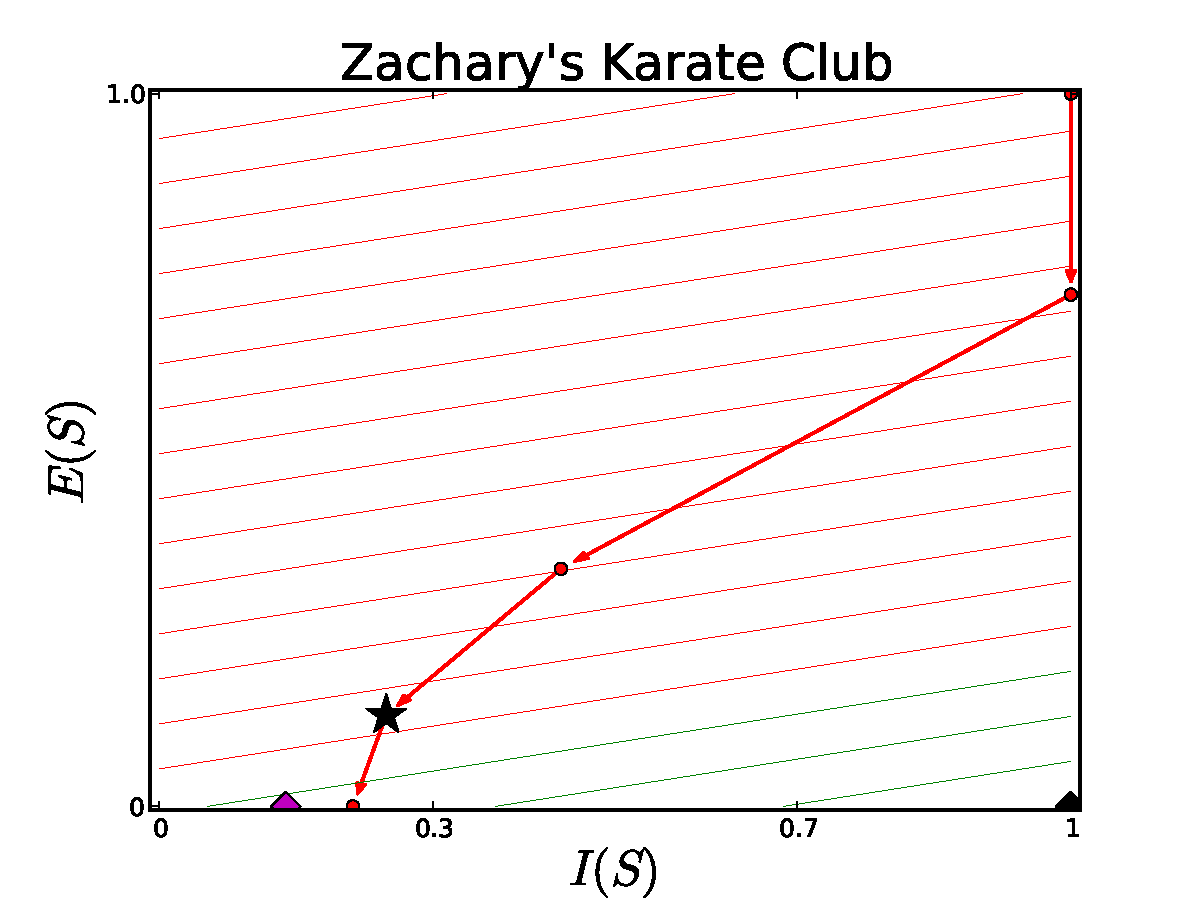
\includegraphics[width=2.8in]{Figures/linear_sets_karate}
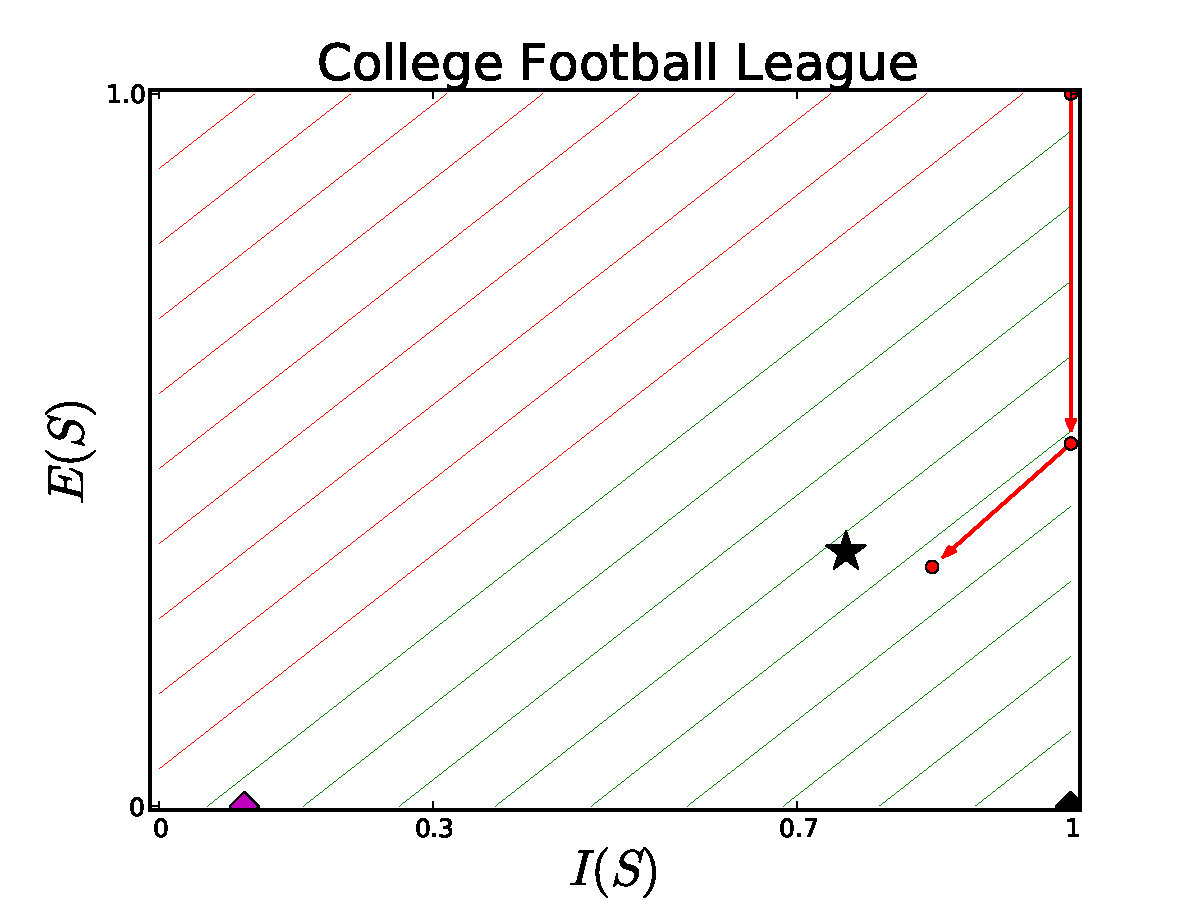
\includegraphics[width=2.8in]{Figures/linear_sets_cfl}
\caption{Linearity for sets of communities compared to Known Solutions (the black stars).   Linearity produces sets of communities with better values of internal and external density. In depth analysis is provided in Figure: \ref{fig:karate_comparison}.}
\label{fig:linear_set_known}
\end{figure}

\begin{figure}[!h]
\centering
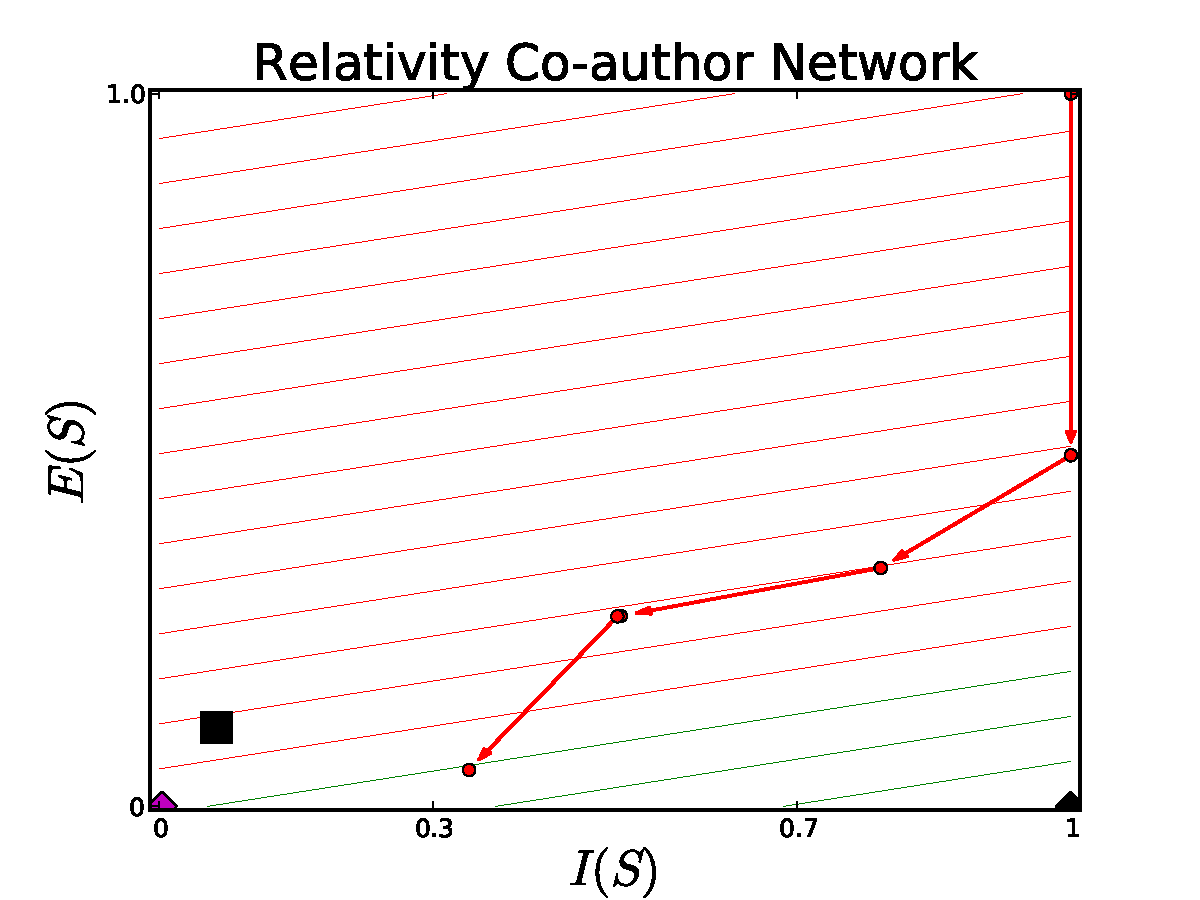
\includegraphics[width=2.8in]{Figures/linear_sets_relativity}
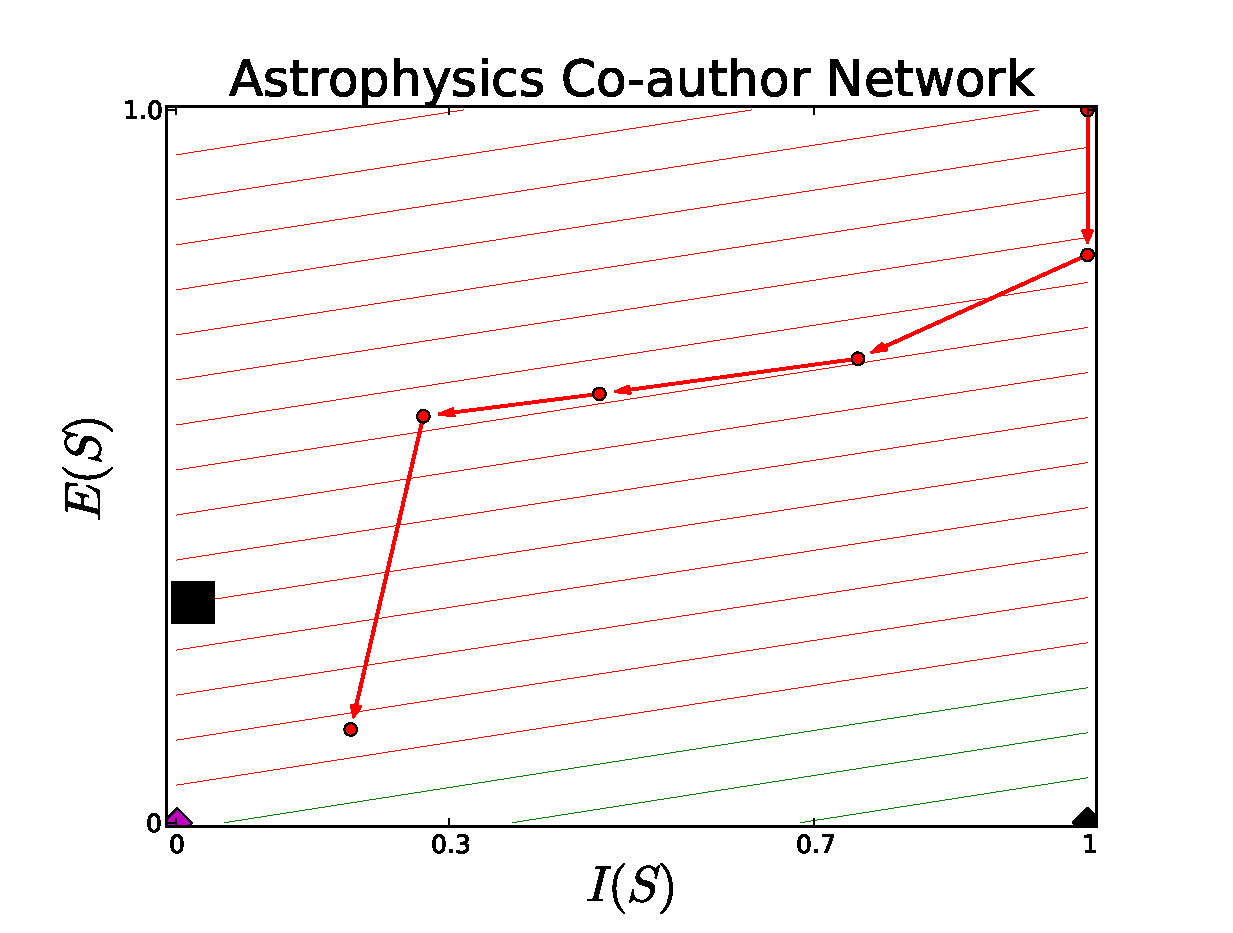
\includegraphics[width=2.8in]{Figures/linear_sets_astro}
\caption{The $I(S)$, $E(S)$ values produced by modularity are provided by black squares.  The linearity path is traced in red.  The first segment corresponds to finding maximal cliques, the middle segments correspond to improvements in the partition due to the Louvain algorithm.  The last segment is from expanding the partitions to produce overlapping communities. In both cases linearity produces sets of communities with better internal and external density values.}
\label{fig:linear_set}
\end{figure}




\chapter{Parallel Community Detection}

The previously covered algorithms for metric maximization is one train of thought

\section {Introduction of Properties and Statistical Significance}

\section{Algorithm}

\subsection{Seeds}

\subsection{Expansion}

\section{Probability of Correctness}

\section {Performance}



\chapter{Case Studies of Networks}
\label{ch:datasets}

So far we have been developing algorithms.  Here, we show how those algorithms perform on a variety of networks.


\section{Known Community Comparisons}

We cover in depth community detection performance on two networks with known community structure.

\subsection{Karate Club Network}

The Karate Club Network represents a set of students belonging to a karate club.  Zachary studied the students in \cite{zachary} and found that students interacted with each other outside of the club's practice times.  In our representation the students are the nodes and their interactions are the edges.  In the course of Zachary's observations, the club split into two groups that wanted to practice seperately.  We consider the two groups the club split into to be the known communities.  We now compare the communities found by different detection methods with the known communities in Figure \ref{fig:karate_comparison}.

\begin{figure}[tb]
\centering
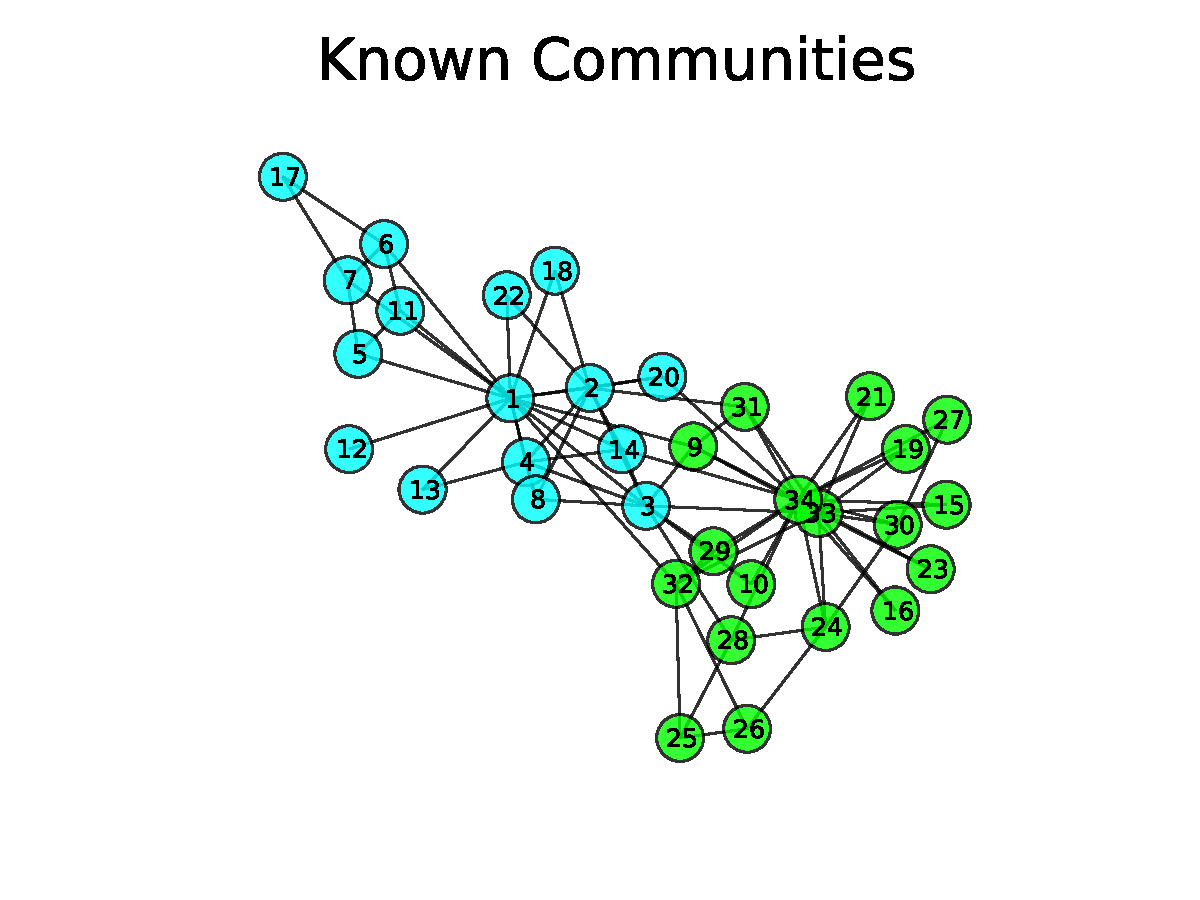
\includegraphics[width=2.8in]{Figures/karate_known_plots}
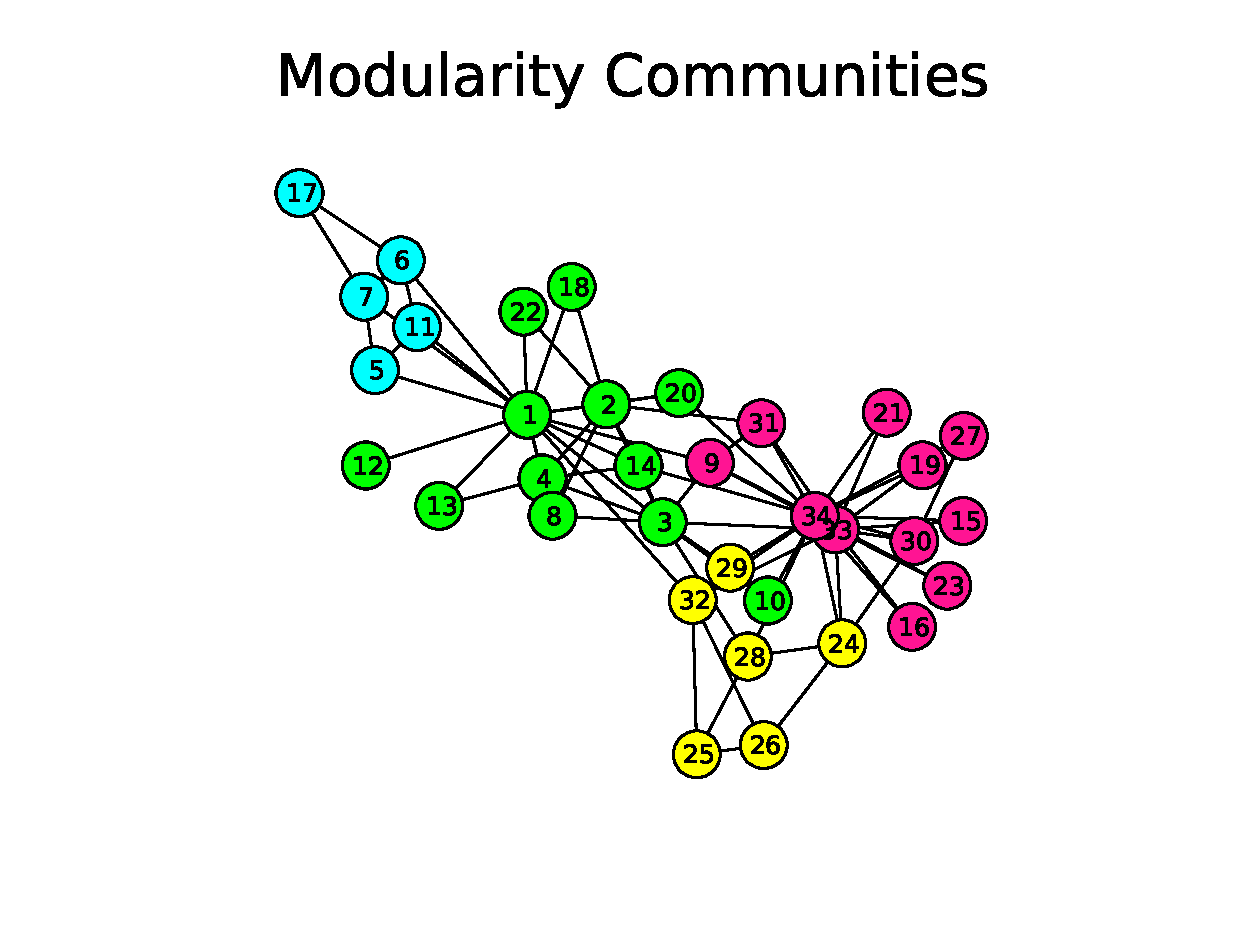
\includegraphics[width=2.8in]{Figures/karate_module_plots}
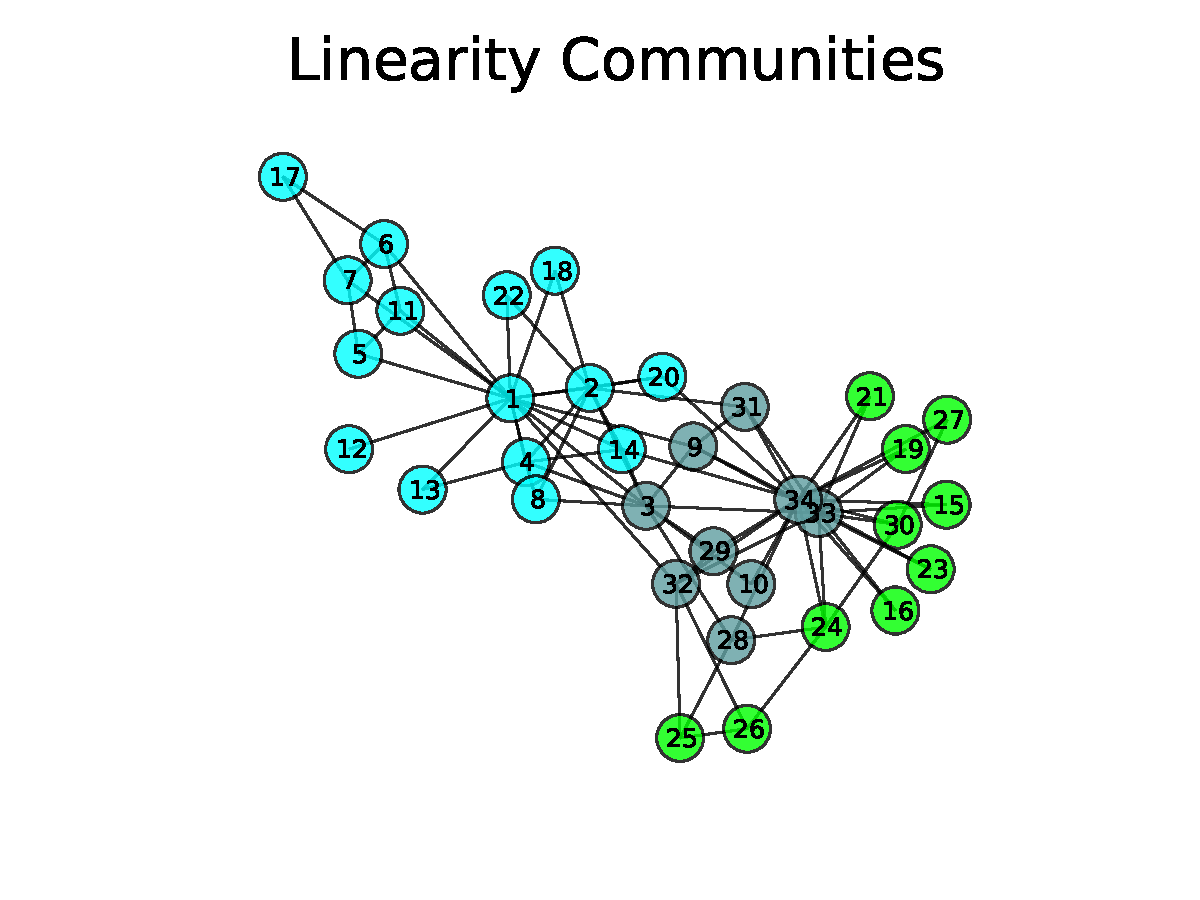
\includegraphics[width=2.8in]{Figures/karate_linear_plots}
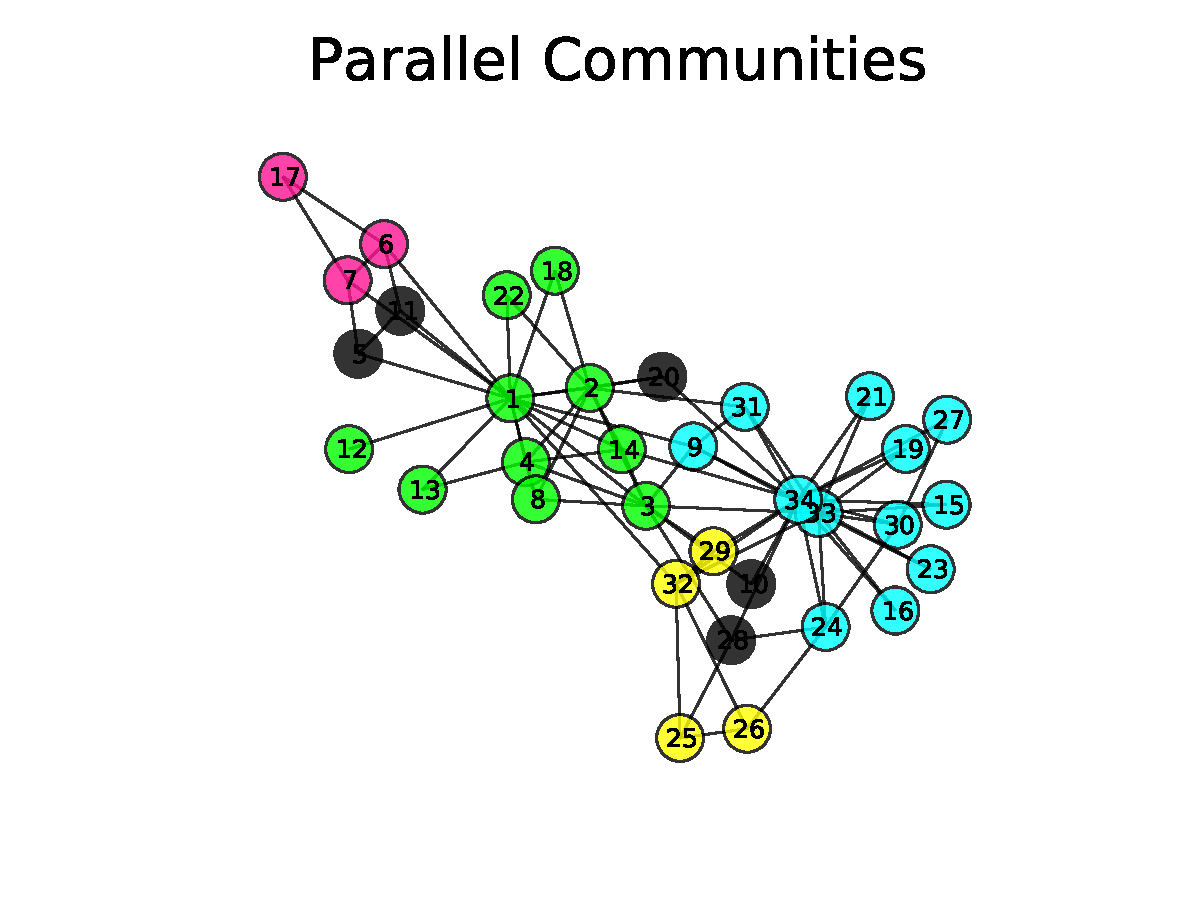
\includegraphics[width=2.8in]{Figures/karate_parallel_plots}
\caption{Communities produced by the different community detection methods, communities are marked by coloration.  Linearity produces two communities with the overlap colored in grey.  Parallel produces four communities with four nodes in black not belonging to any community.}
\label{fig:karate_comparison}
\end{figure}


\begin{table}[!h]
\centering
\begin{tabular}{c|ccc}
Communities From & $I(S)$ & $E(S)$ & $|S|$ \\ \hline
Known & $0.25$ & $0.13$ & $2$\\
Modularity & $0.39$ & $0.27$ & $4$\\
Linearity &$0.21$ & $0.0$ & $2$ \\
Parallel &$0.43$ & $0.35$ & $4$\\
\end{tabular}
\caption{Internal Density, External Density, and number of communities for the set of communities returned by each detection method on the Karate Club network.}
\label{tbl:karate_all}
\end{table}


Each of the detection methods produces different sets of communities, each with its own merit.  Compared to the known communities, the communities produced by linearity are the most similar.  Linearity produces two communities with an overlap.  Within the network there is a set of centerally connected nodes, these are the ones in the overlap.  Maximizing modularity produces four communities.  Two of the communities are large portions of the two known communities.  The additional two communities are more independent and near clique like.  Parallel produces four communities that are subsets of the communities produced by maximizing modularity.  Parallel does not classify five nodes, marked in black.  These nodes have exactly two edges, each going to a different community.  These nodes do not to have a statistically strong connection to any community.



\subsection{College Football Network}

The college football network represents the $115$ collegiate football teams and their games.  The nodes are the teams and the edges represent the two teams played a game.  The collegiate teams are split into divisional conferences, we consider these to be the known communities.  For the games, a team must play nearly every member of its conference.  Additionally, each team plays teams from other conferences.  If team $A$ belongs to a conference with only a few teams, then $A$ must play more teams from other conferences than a team within a larger conference.  This makes large conferences easy to detect and smaller conferences harder to detect.  

\begin{table}[!h]
\centering
\begin{tabular}{c|ccc}
Communities From & $I(S)$ & $E(S)$ & $|S|$ \\ \hline
Known & $0.75$ & $0.36$ &  $12.0$\\
Modularity & $0.68$ & $0.29$ & $10.0$\\
Linearity &$0.85$ & $0.34$ & $13.0$ \\
Parallel &$0.87$ & $0.35$ &  $13.0$\\
\end{tabular}
\caption{Internal Density, External Density, and number of communities for the set of communities returned by each detection method on the CFL network.}
\label{tbl:football_all}
\end{table}

\begin{figure}[tb]
\centering
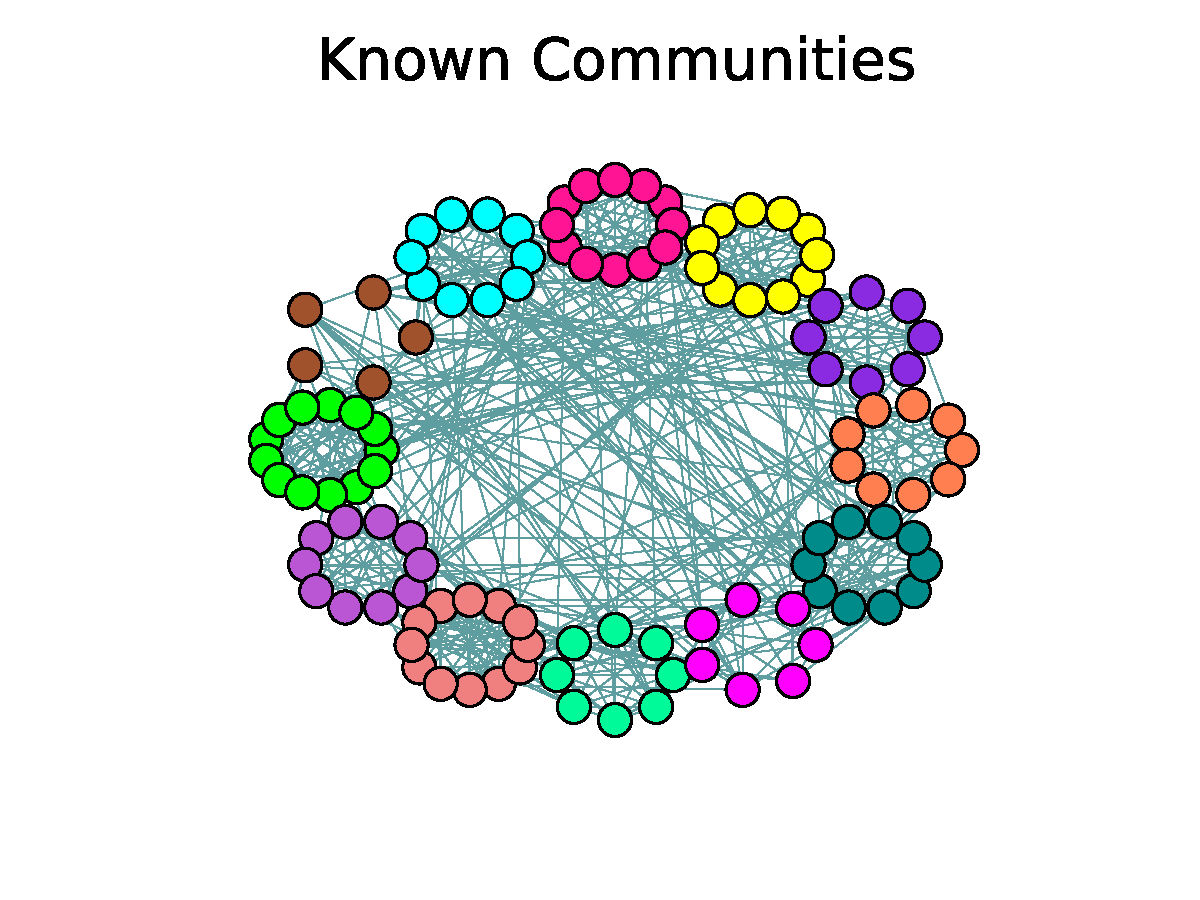
\includegraphics[width=2.8in]{Figures/football_known_plots}
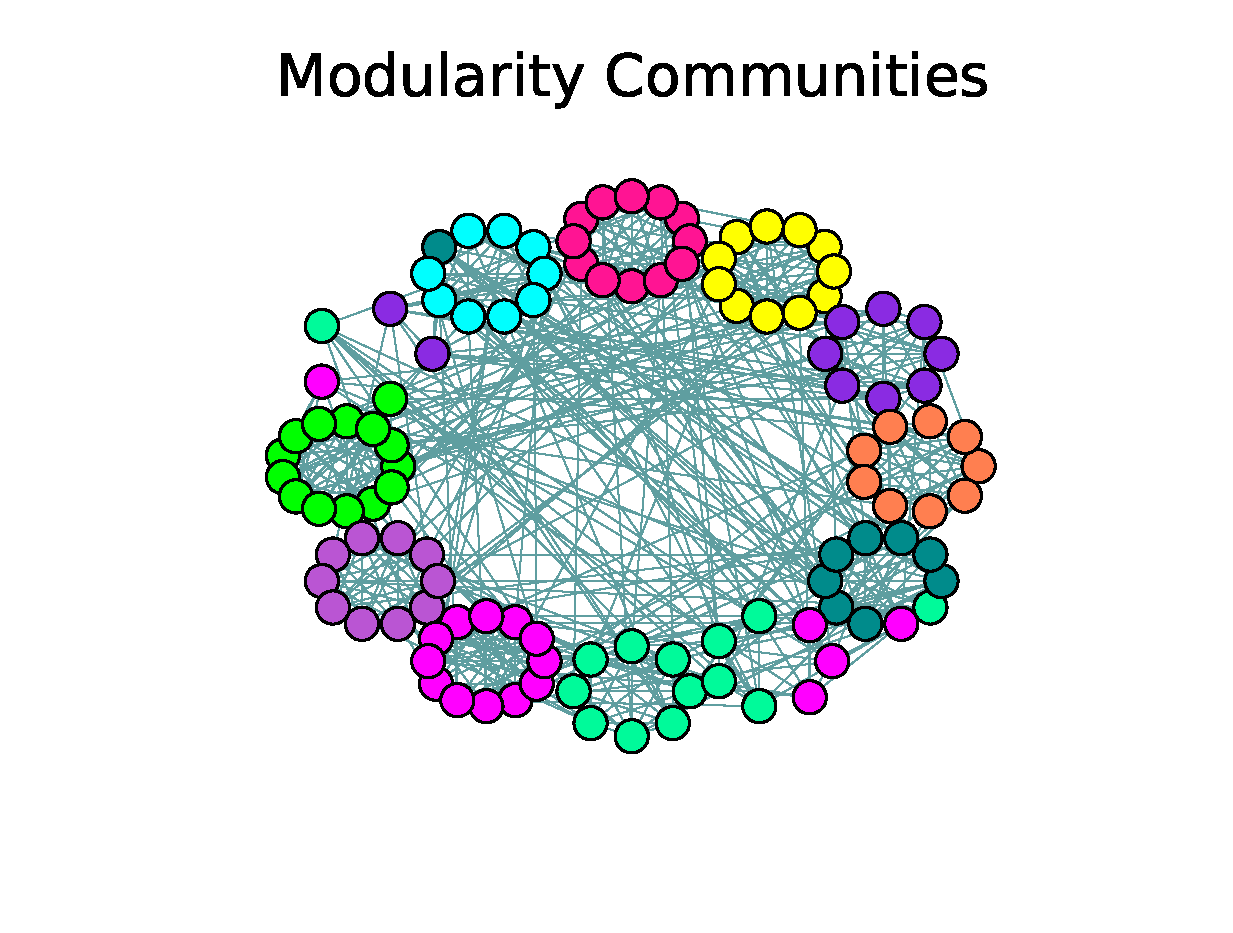
\includegraphics[width=2.8in]{Figures/football_module_plots}
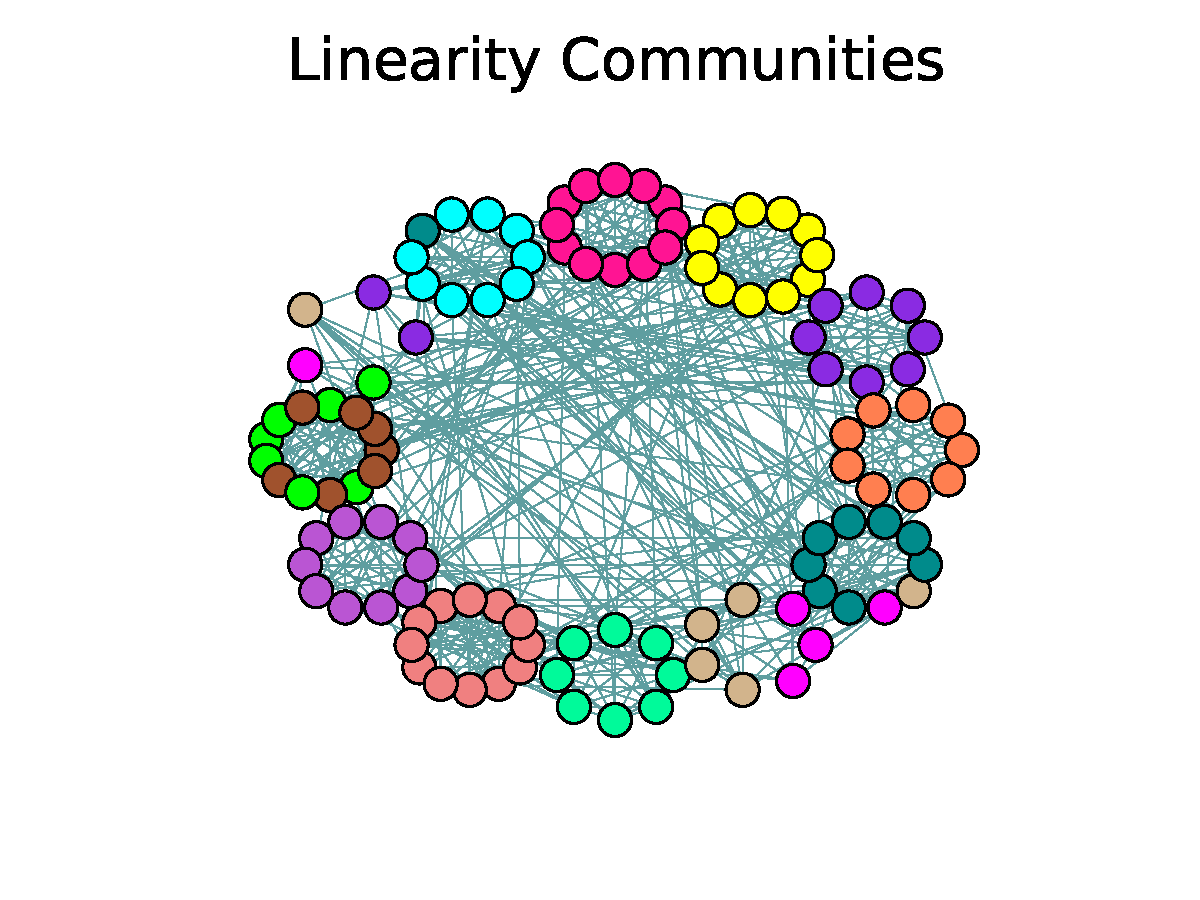
\includegraphics[width=2.8in]{Figures/football_linear_plots}
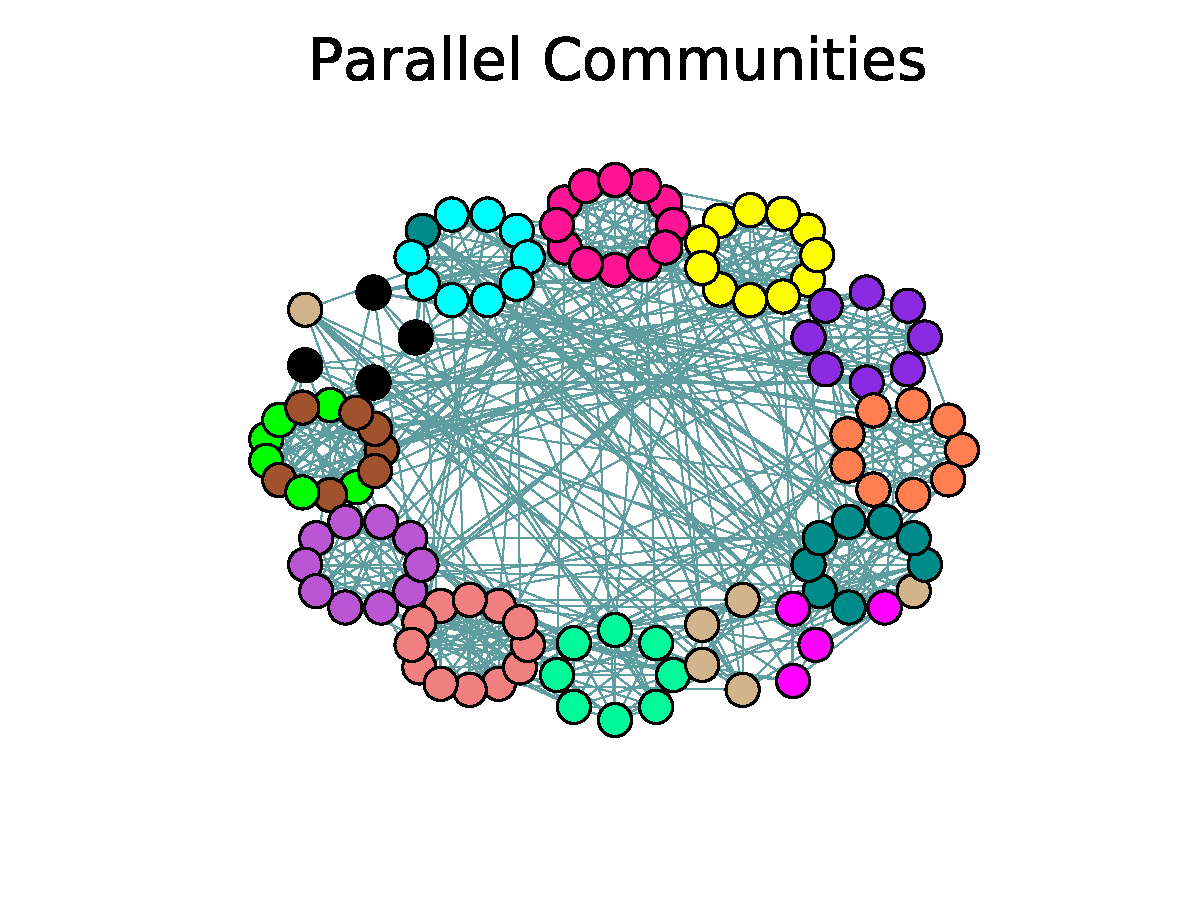
\includegraphics[width=2.8in]{Figures/football_parallel_plots}
\caption{Different solutions produced by the different community detection methods, communities are marked by coloration.  }
\label{fig:football_comparison}
\end{figure}

The communities returned by different detection methods are in Figure \ref{fig:football_comparison}.  There are twelve conferences and we plot each at an hour on a clock face.  Each color represents a different community.  For a majority of the nodes all detection methods produce the same communities.  The smallest conferences are located at five o'clock and ten.  Each detection method breaks these conferences up and handles their nodes in a different way.  Modularity places each node another conference.  The nodes from the five o'clock conference are incorporated into the six and seven o'clock conferences.  Linearity and parallel create two communities for the split five o'clock conference.  Parallel does not classify four of the nodes, in black, in the ten o'clock conference.  These nodes do not have a strong connection to another community.  The last difference is that linearity and parallel break the nine o'clock conference into two communities.  Overall, modularity deviated from the known communities by creating fewer communities to cover more of the edges.  Linearity and parallel deviated from the known communities by creating more and denser communities.



\section{Collaboration Networks}


\subsection{Astrophysics}

\subsection{Condensed Matter}

\subsection{High Energy Physics}

\subsection{General Relativity}



\section{Enron Email Network}

\section{Epinions Social Network}

\section{Gnutella P2P Network}

\section{Physics Citation Network}

\section{Web Graphs}

\subsection{Berkeley Webpage}

\subsection{Google}


\section{Wiki Network}

\subsection{Communication Network}

\subsection{Election Voting Network}



\section{Amazon Product Network}

\chapter{Evolution of Communities}


\chapter{Conclusions}

Above we have provided an indepth look at the details.  Here we provide the summation of our results.

Finding communities is always a tradeoff.  In metric based approaches between internal density and external sparsity.  In significance based approaches the tradeoff is between specificity and sensitivity.

The number of communities a node belongs to follows a power law distribution.

Communities in citation networks evolve from a unioning of previous topics.  However, not all papers that union topics produce successful communities.


\appendix
\chapter{Chapter 1 of appendix}
Appendix chapter 1 text goes here

\bibliography{thesis}

\end{document}

